\subsection{MoE 并行性的挑战}\label{sec:moe-parallelism-challenge}

传统的并行策略是为密集的 Transformer 设计的。 MoE 模型具有根本不同的计算模式，需要新的并行维度、专家并行 (EP)，并且在将 EP 与现有策略相结合时会带来独特的挑战。

\subsubsection{MoE 的并行悖论}\label{sec:parallelism-paradox}

\begin{figure}[t]
    \centering
    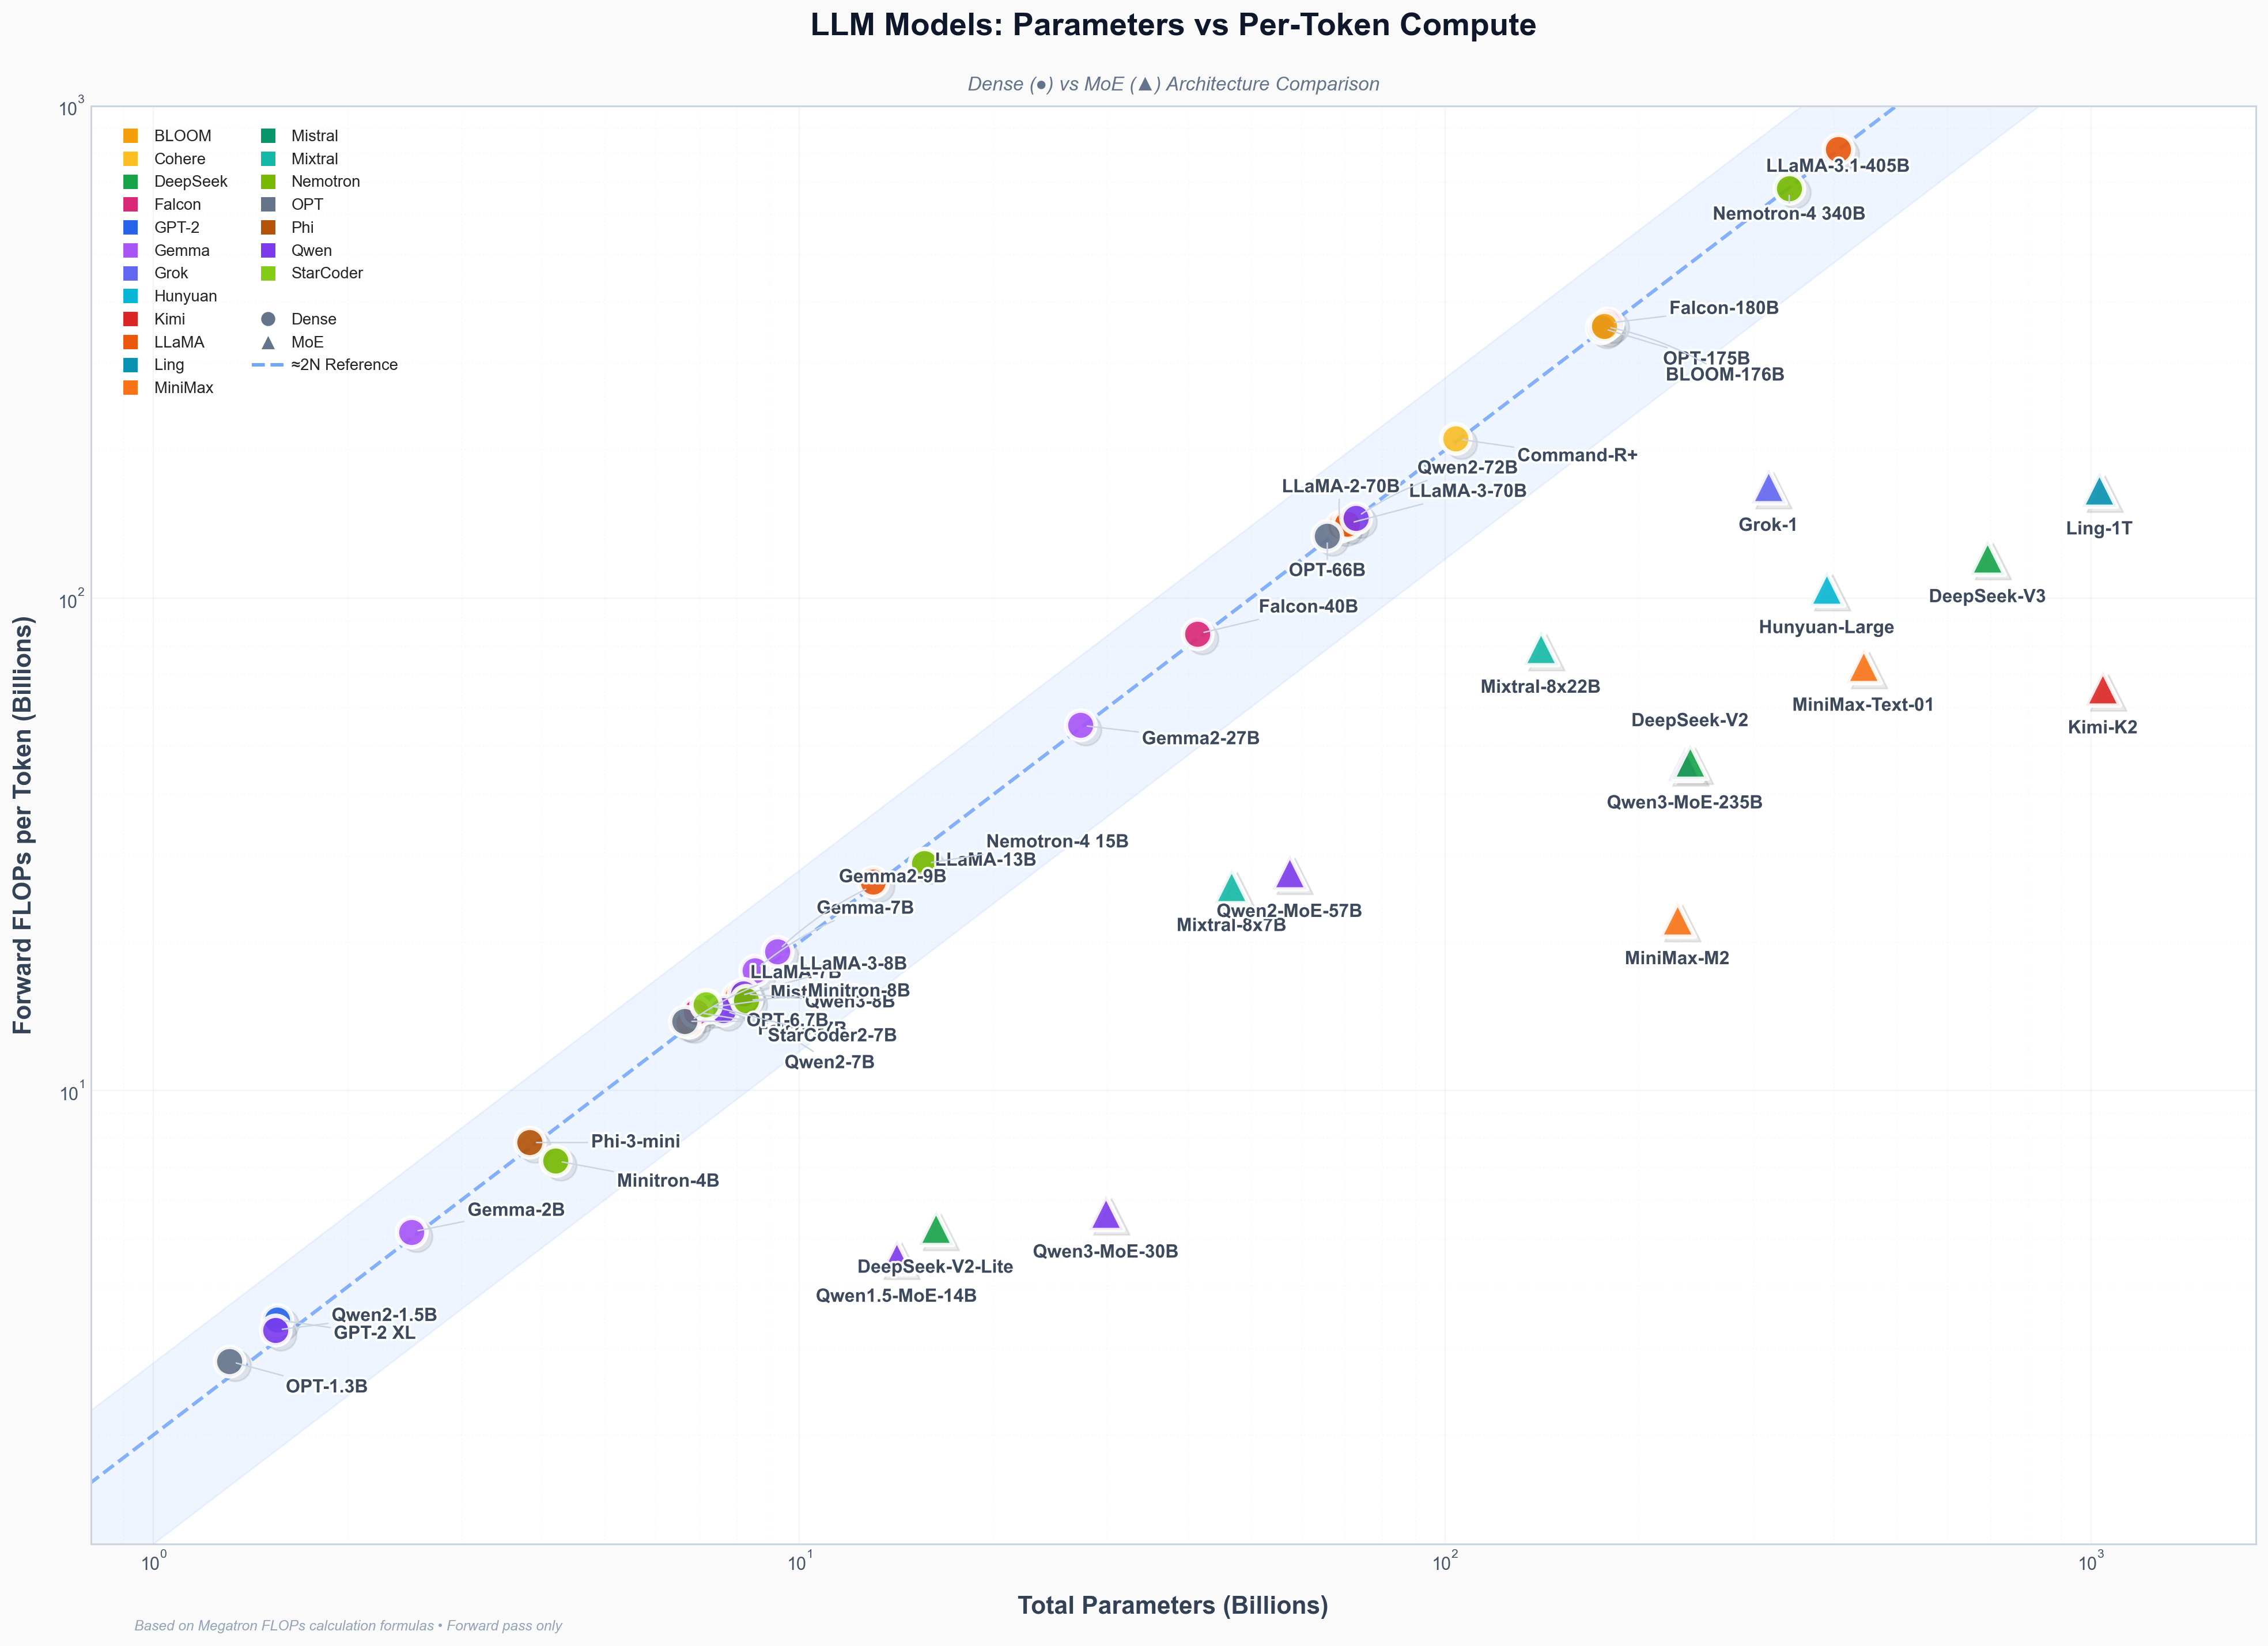
\includegraphics[width=0.95\textwidth]{figures/llm_comparison.png}
    \caption{密集模型与 MoE 模型参数/计算缩放。}
    \label{fig:parallelism-paradox}
\end{figure}

\Figref{fig:parallelism-paradox} 通过绘制总参数与 \emph{向前} 主要法学硕士的每个代币的失败次数。密集模型（圆圈）遵循 $\approx$2N 参考线，展示 \emph{良性循环} 随着规模的扩大：增加参数需要更多的 GPU 来存储内存，但更多的参数也意味着每个令牌的计算量更大。由于计算量随着模型大小的增加而增长，因此通信在每个步骤中所占的份额较小，从而保持 MFU 稳定。

MoE 模型（三角形）打破了这个循环。它们明显低于 2N 线，以每个代币更少的 FLOP 实现同等的功能。考虑基本的不对称性：

\begin{center}
\begin{tabular}{lccc}
\toprule
\textbf{模型} & \textbf{总参数} & \textbf{活动参数} & \textbf{比率} \\
\midrule
Llama-70B（密集） & 70B & 70B & 1:1 \\
DeepSeek-V3（教育部） & 685B & 37B & \textbf{18:1} \\
\bottomrule
\end{tabular}
\end{center}

{\footnotesize \textbf{笔记：} DeepSeek-V3 包含 671B 主模型权重和 14B 多令牌预测 (MTP) 模块权重（总共 685B）。该表显示了包括 MTP 在内的总模型参数。}

DeepSeek-V3有18个$\times$ 比其主动计算建议的参数更多，可见于 \Figref{fig:parallelism-paradox} 作为 DeepSeek-V3 位置与等效参数密集模型所在位置之间的差距。这创建了一个 \emph{复合效应}:

\begin{enumerate}
    \item \textbf{内存增长很快}，强制分布在多个 GPU 上：全部 $E$ 专家的参数、梯度和优化器状态必须驻留在内存中，并且更大的top-$k$ 通过令牌复制进一步增加激活内存。
    \item \textbf{更多沟通}：通过 EP 分配专家引入了全对全流量，其流量随 $K$ （每个令牌被发送到 $K$ EP 级别的专家）。
    \item \textbf{但计算量仍然很低}：每个代币的 FLOP 数仅可扩展 $N_{\text{active}}$ ($\propto K$）， 不是 $N_{\text{total}}$ ($\propto E$），导致计算量不足以与不断增长的通信重叠。
\end{enumerate}

结果： \textbf{教育部培训从根本上讲是与沟通相关的} 除非并行性是专门针对这种不对称性而设计的。这不是程度的问题，而是程度的问题。这是一个 \emph{质的差异} 来自密集模型。

\subsubsection{传统并行策略}\label{sec:traditional-parallelism}

Dense Transformer 训练通常结合四种并行策略：

\textbf{张量并行度 (TP)} 沿隐藏维度跨 GPU 分片权重矩阵 \cite{shoeybi2020megatronlmtrainingmultibillionparameter}。每个GPU 计算部分结果，然后AllGather 或ReduceScatter 集体组合结果。当矩阵大到足以抵消通信开销时，TP 效果很好。

\textbf{管道并行度 (PP)} 在 GPU 上按层分割模型 \cite{huang2019gpipe,narayanan2019pipedream,shoeybi2020megatronlmtrainingmultibillionparameter,qi2023zerobubblepipelineparallelism,qi2024pipelineparallelismcontrollablememory,zhang2022chimera,guan2025pipeoptimensuringeffective1f1b}。微批次流经管道，阶段之间进行点对点通信。 PP 引入了管道气泡（边界处的空闲时间）和 P2P 通信开销，但跨节点的扩展性比 TP 更好。

\textbf{数据并行性 (DP)} 跨 GPU 复制模型，每个 GPU 处理不同的数据批次 \cite{shallue2019measuringeffectsdataparallelism,bai2022moderndistributeddataparallellargescale}。梯度通过 AllReduce 同步。 DP 很简单，但需要每个 GPU 保存完整的模型。

\textbf{上下文并行性 (CP)} \cite{korthikanti2023sequence,liu2023ringattention,jacobs2023deepspeedulysses} 沿序列维度跨 GPU 划分输入序列。每个 GPU 处理序列的连续块，仅在注意力计算时需要通信，其中令牌必须跨越块边界。 CP 对于长上下文训练至关重要，其中激活记忆与序列长度呈二次方缩放。

\textbf{为什么传统的并行性对于 MoE 来说失败了：}

\begin{itemize}
    \item \textbf{教育部专家的 TP}：专家隐藏尺寸小；应用 TP 会创建更小的分片，降低计算效率，同时增加通信在总时间中所占的份额。高TP可以有效分配注意力，但是 \emph{伤害} 教育部。
    \item \textbf{PP与众多专家}：MoE 模型具有大量参数，如果单独使用 PP，则需要许多管道阶段。这会产生过多的管道气泡并降低吞吐量。
    \item \textbf{单独DP}：DP 在每个 GPU 上复制完整模型。对于万亿参数模型来说，这是不可能的，因为DP不能划分参数，只能划分数据。
\end{itemize}

\subsubsection{专家并行性：第五维度}\label{sec:expert-parallelism}

传统并行分区 \emph{层数} （PP）， \emph{权重矩阵} （TP）， \emph{顺序} （CP），或 \emph{数据} （DP）。但教育部有一个独特的结构： \textbf{专家是独立的子网络}。这实现了第五个并行维度，用于分区 \emph{专家本身} 跨 GPU。

\textbf{专家并行 (EP)} 跨 GPU 分配专家 \cite{lepikhin2020gshard}。 EP 度等于 $E$，每个GPU持有 $E/\text{EP}$ 专家。前向传播过程如下：

\begin{enumerate}
    \item \textbf{路线}：路由器选择top-$k$ 每个代币的专家。
    \item \textbf{派遣}：所有对所有的通信将令牌发送到持有其指定专家的 GPU。
    \item \textbf{计算}：每个 GPU 仅使用其本地专家来处理令牌。
    \item \textbf{结合}：所有对所有通信将结果返回到原始 GPU。
\end{enumerate}

\textbf{EP 独特的权衡}:
\begin{itemize}
    \item \textbf{沟通}: 全体集体。交易量与代币数量有关，而不是与专家数量有关。
    \item \textbf{计算}：每个 GPU 运行较少的专家，但每个专家处理其 \emph{满的} 隐藏维度。
    \item \textbf{记忆}：更高的 EP = 每个 GPU 更少的专家 = 更低的内存压力。
\end{itemize}

EP 提供两个主要优势（\figref{fig:expert-parallelism-overview}）。首先，将来自不同 GPU 的令牌分组到单个专家会增加计算强度，从而提高 GEMM 效率。其次，随着专家数量的增加，所有人对所有人的通信量保持不变；仅 GPU 数量发生变化。

\begin{figure}[ht]
    \centering
    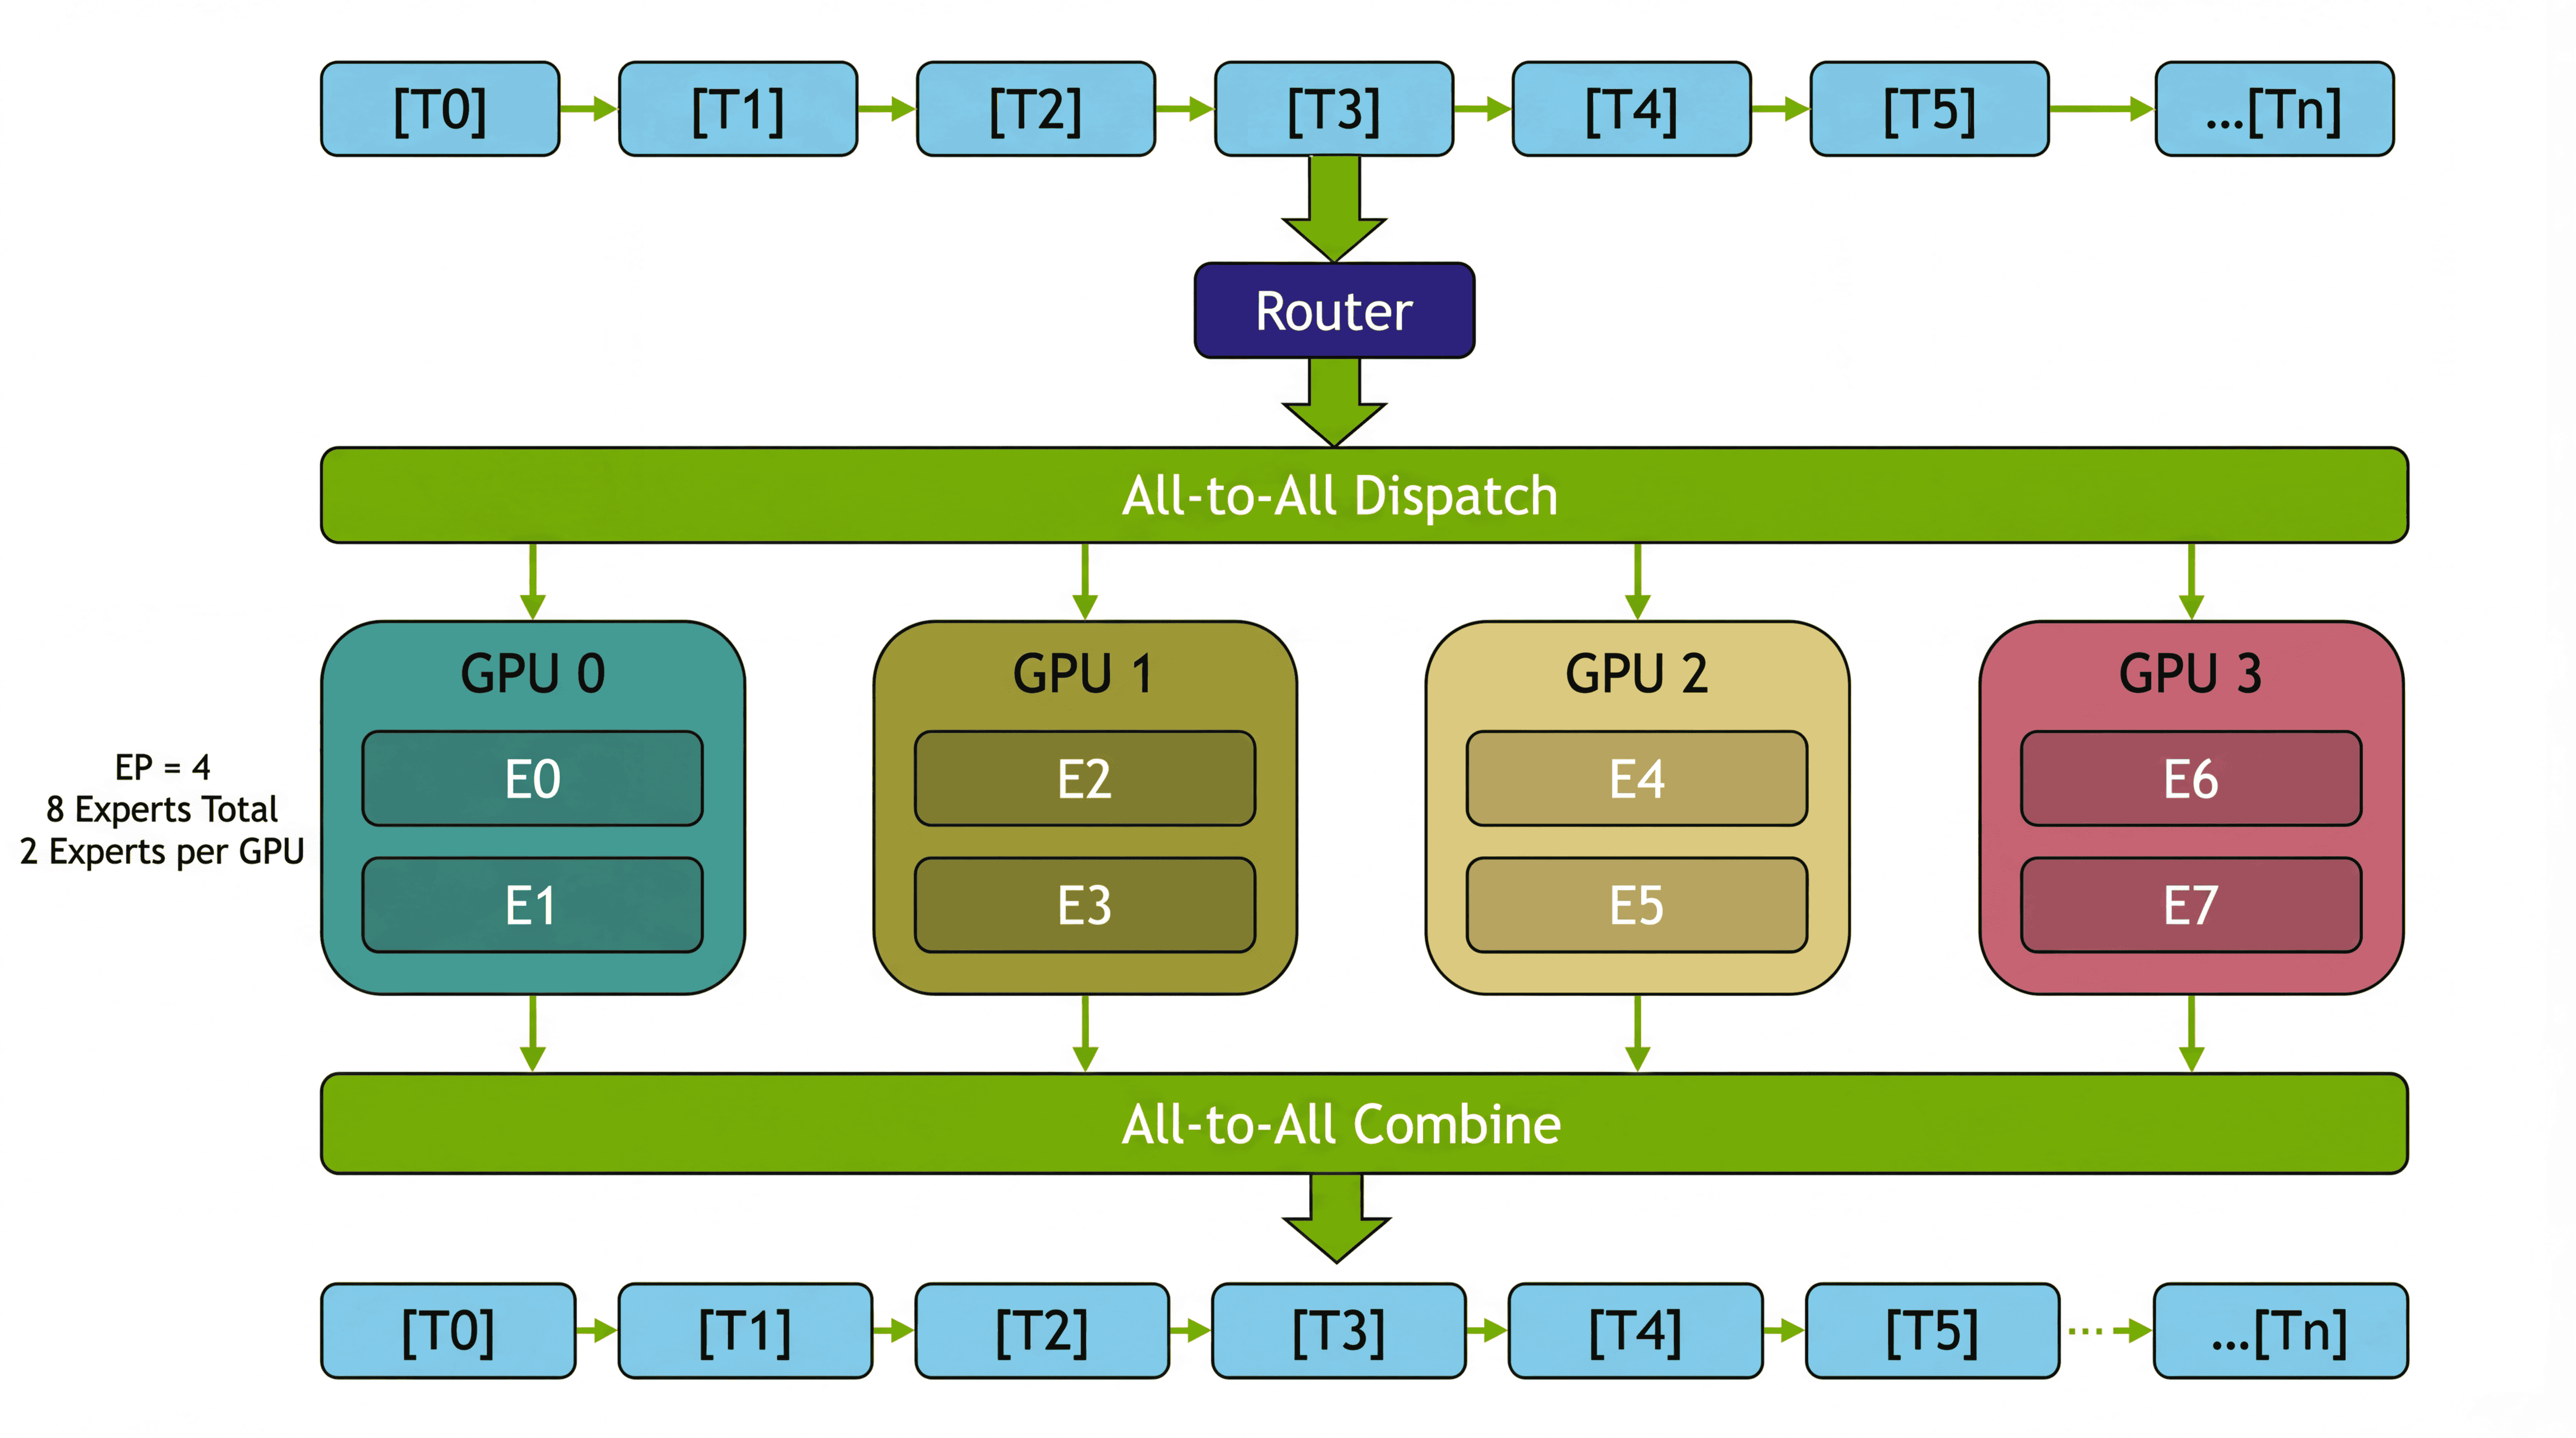
\includegraphics[width=0.9\textwidth]{figures/plots/expert_parallelism_overview_draft.png}
    \caption{专家并行 (EP) 将专家分布在 GPU 上。全面通信将代币发送给指定的专家并合并结果。}
    \label{fig:expert-parallelism-overview}
\end{figure}

\textbf{但仅 EP 还不够。} EP仅适用于MoE层；注意力层没有专家，仍然需要 TP、CP 或其他策略。此外，这两种层类型都需要 Pipeline Parallelism 来进一步划分模型参数以进行大规模 MoE 训练。这种异质性造成了接下来讨论的密集稀疏不匹配。

\subsubsection{EP 与传统并行性相结合的挑战}\label{sec:combining-parallelism}

单个 Transformer 块包含 \textbf{两种根本不同的计算模式} \cite{Singh_2023}，总结如表~\ref{tab:dense-sparse-comparison}:

\begin{table}[ht]
\centering
\caption{对比单个 Transformer 块内注意力层和 MoE 层的并行性要求。}
\label{tab:dense-sparse-comparison}
\begin{tabular}{lp{0.4\textwidth}p{0.4\textwidth}}
\toprule
\textbf{方面} & \textbf{注意（密集）} & \textbf{教育部（稀疏）} \\
\midrule
计算 & 每个令牌都关注所有其他令牌 & 每个令牌路由到 $K$ 的 $E$ 专家 \\
TP & 大型 QKV 矩阵受益于高 TP & 每个专家的规模较小使得高 TP 适得其反 \\
CP & 长序列受益于高 CP & 无顺序依赖性； CP无所谓 \\
EP & 不适用（无专家） & 对于分配许多专家来说至关重要 \\
\bottomrule
\end{tabular}
\end{table}

\textbf{密集-稀疏不匹配。} 传统框架的力量 \emph{一} 并行度配置 \emph{两个都} 层类型不同，但它们的最优配置直接冲突：高TP有利于注意力，但会分散专家分片；高 CP 有助于长上下文注意力，但对 MoE 层没有任何好处；高EP对于MoE来说是必要的，但与注意力无关。就像参数计算不匹配一样（小节~\ref{sec:challenges}），这源于 MoE 的稀疏性，但体现在并行配置级别：它是一个 \textbf{结构失配} 密集层和稀疏层的需求之间的关系，而不是调整问题。

之前的 MoE 框架将 EP 视为 DP 的子维度 \cite{lepikhin2020gshard,fedus2022switchtransformersscalingtrillion}:
\[
\text{World Size} = \text{TP} \times \text{CP} \times \text{PP} \times \text{DP}, \quad \text{where } \text{EP} \subseteq \text{DP}
\]

这种约束的存在是因为框架假设了统一并行性：注意层使用（TP、CP、PP、DP），而 MoE 层只是将 EP 从 DP 组中分离出来。这种设计带来了三个关键挑战：

\textbf{挑战 1：乘法 GPU 要求。} 传统框架需要 $\text{TP} \times \text{CP} \times \text{PP} \times \text{DP}$ 至少需要 GPU。自从EP $\subseteq$ DP，请求EP=8强制DP $\geq$ 8. 结合长序列的 CP=8，最小值变为 $1 \times 8 \times 1 \times 8 = 64$ GPU——即使 Attention 和 MoE 理论上可以共享相同的 8 个 GPU。这提高了教育部培训的准入门槛。

\textbf{挑战 2：强制次优并行。} 由于注意力和 MoE 共享相同的 TP 配置，因此实践者必须在两种次优配置之间进行选择：使用高 TP（例如 TP=8）来有效地对大型注意力矩阵进行分片，这会将小专家分割成低效的分片；或者使用低 TP（例如 TP=1）来保持专家计算效率，这使得注意力层无法并行化。这两种选项都无法实现两种层类型的最佳性能。

\textbf{挑战3：跨节点通信。} 由于 EP 限制在 DP 内，高 EP 通常会迫使所有对所有的通信跨越节点边界，其中带宽为 5--10$\times$ 低于 NVLink。同时，CP注意力通信也可以跨节点。如果无法独立地将 EP 和 CP 映射到高带宽域，通信开销将主导训练时间。

这些挑战不是独立的调优问题。它们源于所有层必须共享一种并行配置的基本假设。 \textbf{问题变成}：我们如何打破这些限制，同时仍然允许每个层类型使用其最佳并行性？

%==============================================================================
% 3.3 Megatron-Core's Solution: Parallel Folding
%==============================================================================
\subsection{Megatron-Core的解决方案：平行折叠和多维框架}\label{sec:parallel-folding}

\textbf{平行折叠} 是威震天核心对密集稀疏不匹配问题的回答。并行折叠不是强迫注意力层和 MoE 层共享相同的并行配置 \textbf{解耦它们的并行映射}，允许每个层类型使用其最佳拓扑 \cite{liu2025moeparallelfoldingheterogeneous}。本节涵盖关键概念和优点；配套论文中描述了并行转换处理和令牌调度设计等实现细节 \cite{liu2025moeparallelfoldingheterogeneous}.

\subsubsection{解耦并行映射}

核心思想很简单： \emph{不要强迫attention和MoE共享并行性}。让每个人独立地使用其最佳配置。

\begin{figure}[ht]
    \centering
    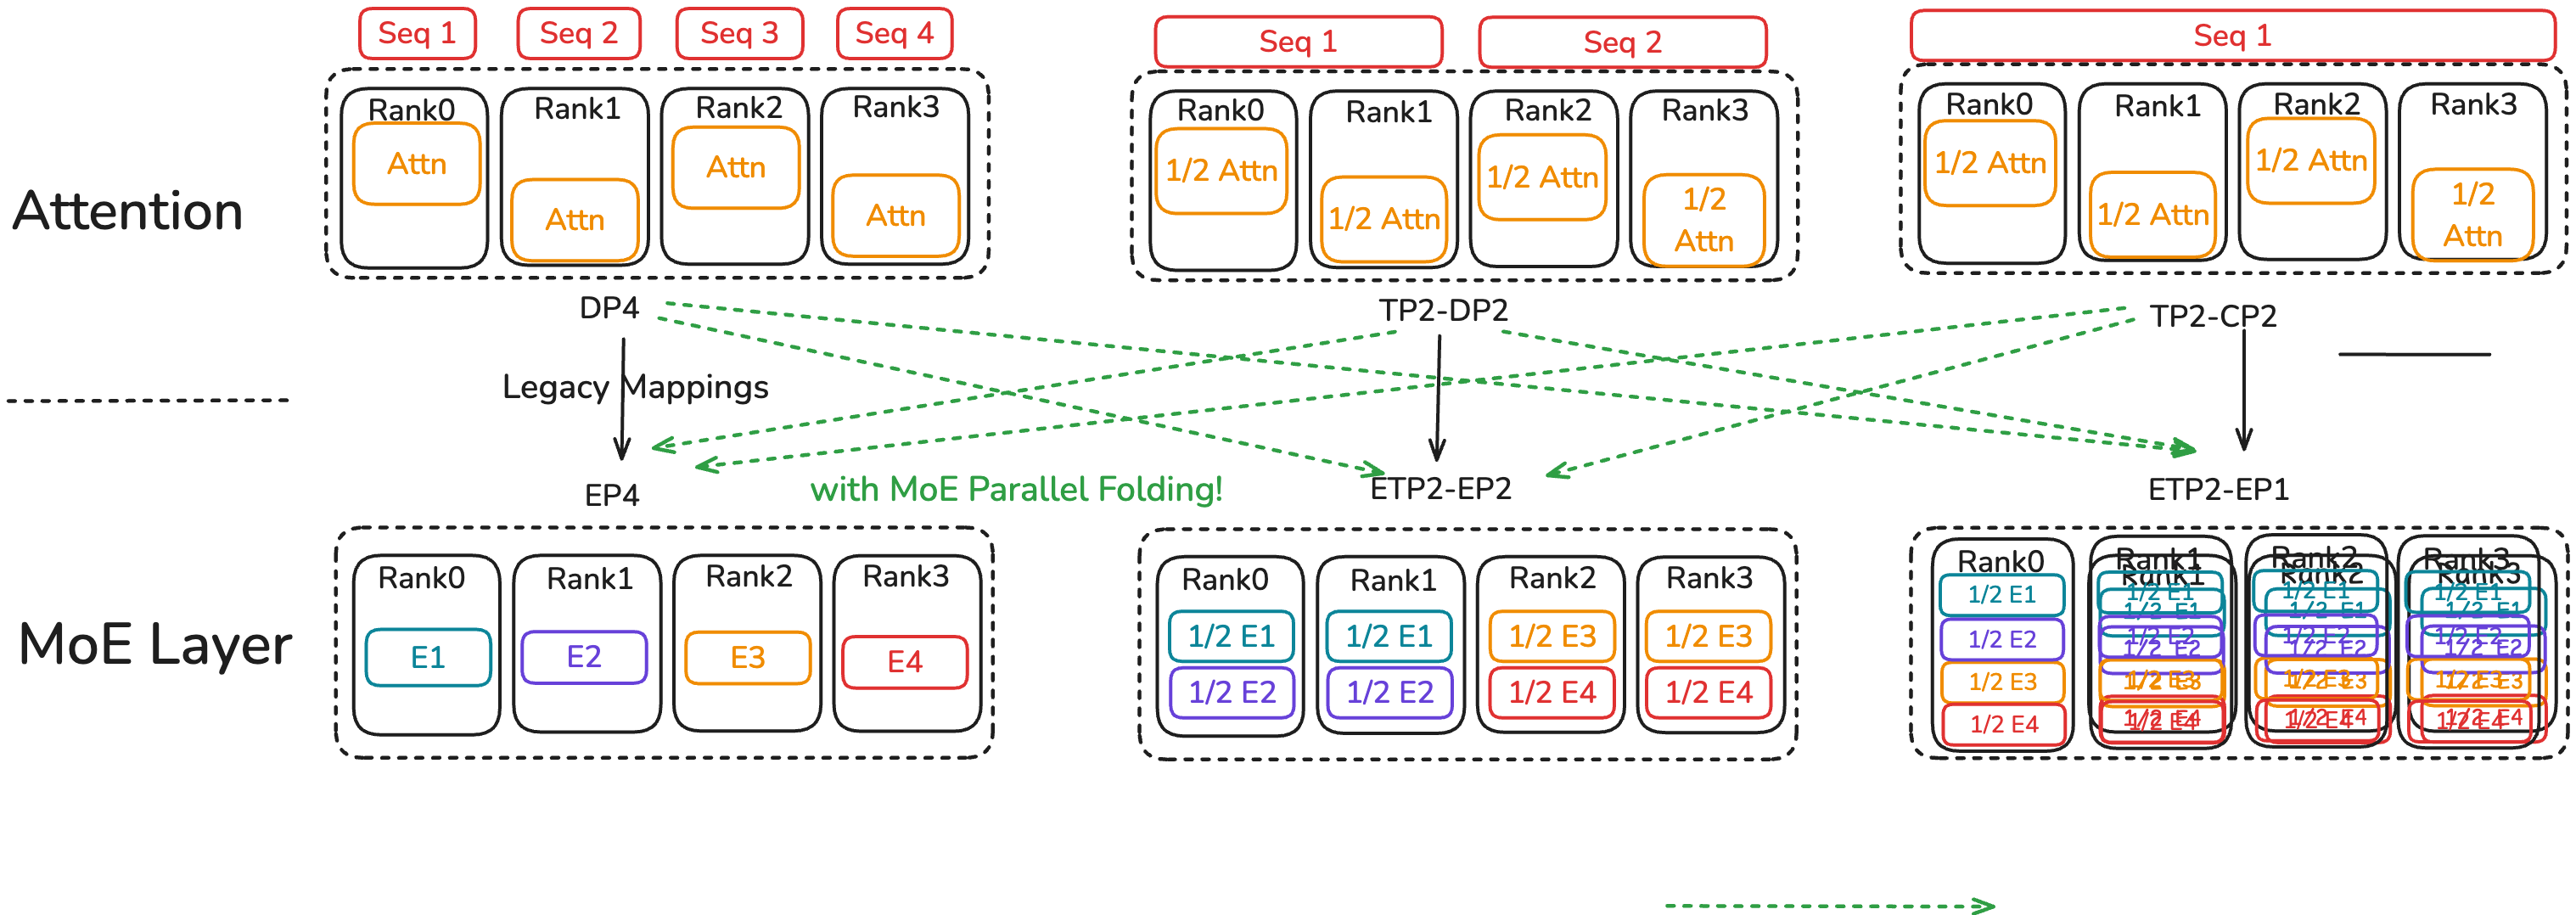
\includegraphics[width=0.9\textwidth]{moe-plots/Parallel-Folding-Paper/MoE_Parallel_Folding-mapping-switch.excalidraw.png}
    \caption{并行映射：传统约束与 MoE 并行折叠解耦。}
    \label{fig:moe-parallel-folding}
\end{figure}

并行折叠为注意力层和 MoE 层引入了单独的并行组：

\begin{itemize}
    \item \textbf{注意力层} 形成小组 $\text{TP} \times \text{CP} \times \text{DP} \times \text{PP}$，针对序列级密集计算进行了优化。
    \item \textbf{教育部层} 形成小组 $\text{ETP} \times \text{EP} \times \text{EDP} \times \text{PP}$，其中 ETP（专家张量并行）和 EDP（专家数据并行）是 MoE 特定的维度。
\end{itemize}

唯一的约束： \textbf{管道并行度 (PP) 必须保持一致} 跨两种布局，以确保正确的梯度流通过模型。
\subsubsection{完整的多维并行堆栈}\label{sec:multi-dim-parallelism}

以并行折叠为基础，Megatron-Core 精心策划了五个并行维度：

\begin{center}
\begin{tabular}{lll}
\toprule
\textbf{方面} & \textbf{适用于} & \textbf{目的} \\
\midrule
TP（张量） & 注意力 & 分片大型 QKV/投影矩阵 \\
CP（上下文） & 注意力 & 分配长序列 \\
DP（数据） & 注意力 & 处理不同批次 \\
PP（管道） & 两个都 & 按层拆分模型（必须一致） \\
\midrule
EP（专家） & 教育部 & 跨 GPU 分配专家 \\
ETP（专家张量） & 教育部 & 专家内部分片（很少使用） \\
EDP​​（专家数据） & 教育部 & 复制专家的吞吐量 \\
\bottomrule
\end{tabular}
\end{center}

\textbf{关键配置原则}:
\begin{itemize}
    \item \textbf{注意力层}：针对大型矩阵（高 TP）和长序列（高 CP）进行优化。
    \item \textbf{教育部层}：针对许多小专家进行优化（高EP，通常ETP=1）。
    \item \textbf{聚丙烯}：两者必须保持一致，以确保正确的数据流。
\end{itemize}

除了上述并行策略之外（\figref{fig:parallel-folding-detailed}），Megatron-Core 的并行折叠框架还集成了分布式优化器和具有 EP 支持的 FSDP，以进一步减少内存占用：

\textbf{分布式优化器+EP。} 每个等级中只有本地专家的权重和梯度；优化器状态在同一 Expert 的副本之间进行分片（通过 EDP）。这消除了非本地专家的冗余优化器内存，并将梯度同步限制在最小组内。

\textbf{FSDP + EP。} 为了实现更高的内存效率，Megatron-Core 的定制 FSDP (Megatron-FSDP) 通过双 DeviceMesh 架构跨数据/专家组完全分片参数、梯度和优化器状态，​​减少内存占用，同时将 AllGather 和 ReduceScatter 与计算重叠。它兼容 TP/EP/CP 和混合精度（BF16、FP8、FP4）。看 \secref{sec:fsdp-ref} 以获得完整的设计。

\subsubsection{平行折叠的好处}

如图所示 \figref{fig:moe-parallel-folding}, MoE平行折叠消除了EP $\leq$ 通过允许 EP 在注意力并行配置的任意子组上“折叠”来限制 DP。这提供了四个关键优势：

\begin{enumerate}
    \item \textbf{打破EP $\leq$ DP约束}：EP 现在可以通过折叠 TP 来超过 DP$\times$CP组。考虑配置为 TP=4、CP=2、DP=8、PP=4（总共 256 个 GPU）的注意力：
    \begin{itemize}
        \item 繁体：EP $\leq$ DP = 8，因此最大 EP 为 8。
        \item 对于平行折叠：MoE 使用 ETP=1、EP=64、EDP=1（相同 PP=4）。 EP“折叠”穿过 TP$\times$CP$\times$DP 组，启用 8$\times$ 更高的专家并行性，同时注意力层保持最佳 TP=4、CP=2 配置。
    \end{itemize}
    
    \item \textbf{降低最低 GPU 要求}：CP=8、EP=8 的传统配置至少需要 64 个 GPU。通过 Folding，CP 和 EP 共享相同的 GPU 组，仅需要 8 个 GPU。
    
    \item \textbf{实现独立优化}：Attention 可以对大型矩阵使用高 TP，而 MoE 使用 ETP=1 以获得完整的专家宽度和更好的 GEMM 效率。
    
    \item \textbf{在 NVLink 域中保持高带宽通信}：CP（用于注意力）和 EP（用于 MoE）全对全通信都可以保留在 NVLink 连接的 GPU 组内，从而避免较慢的跨节点传输。
\end{enumerate}

% fix typo
\begin{figure}[ht]
    \centering
    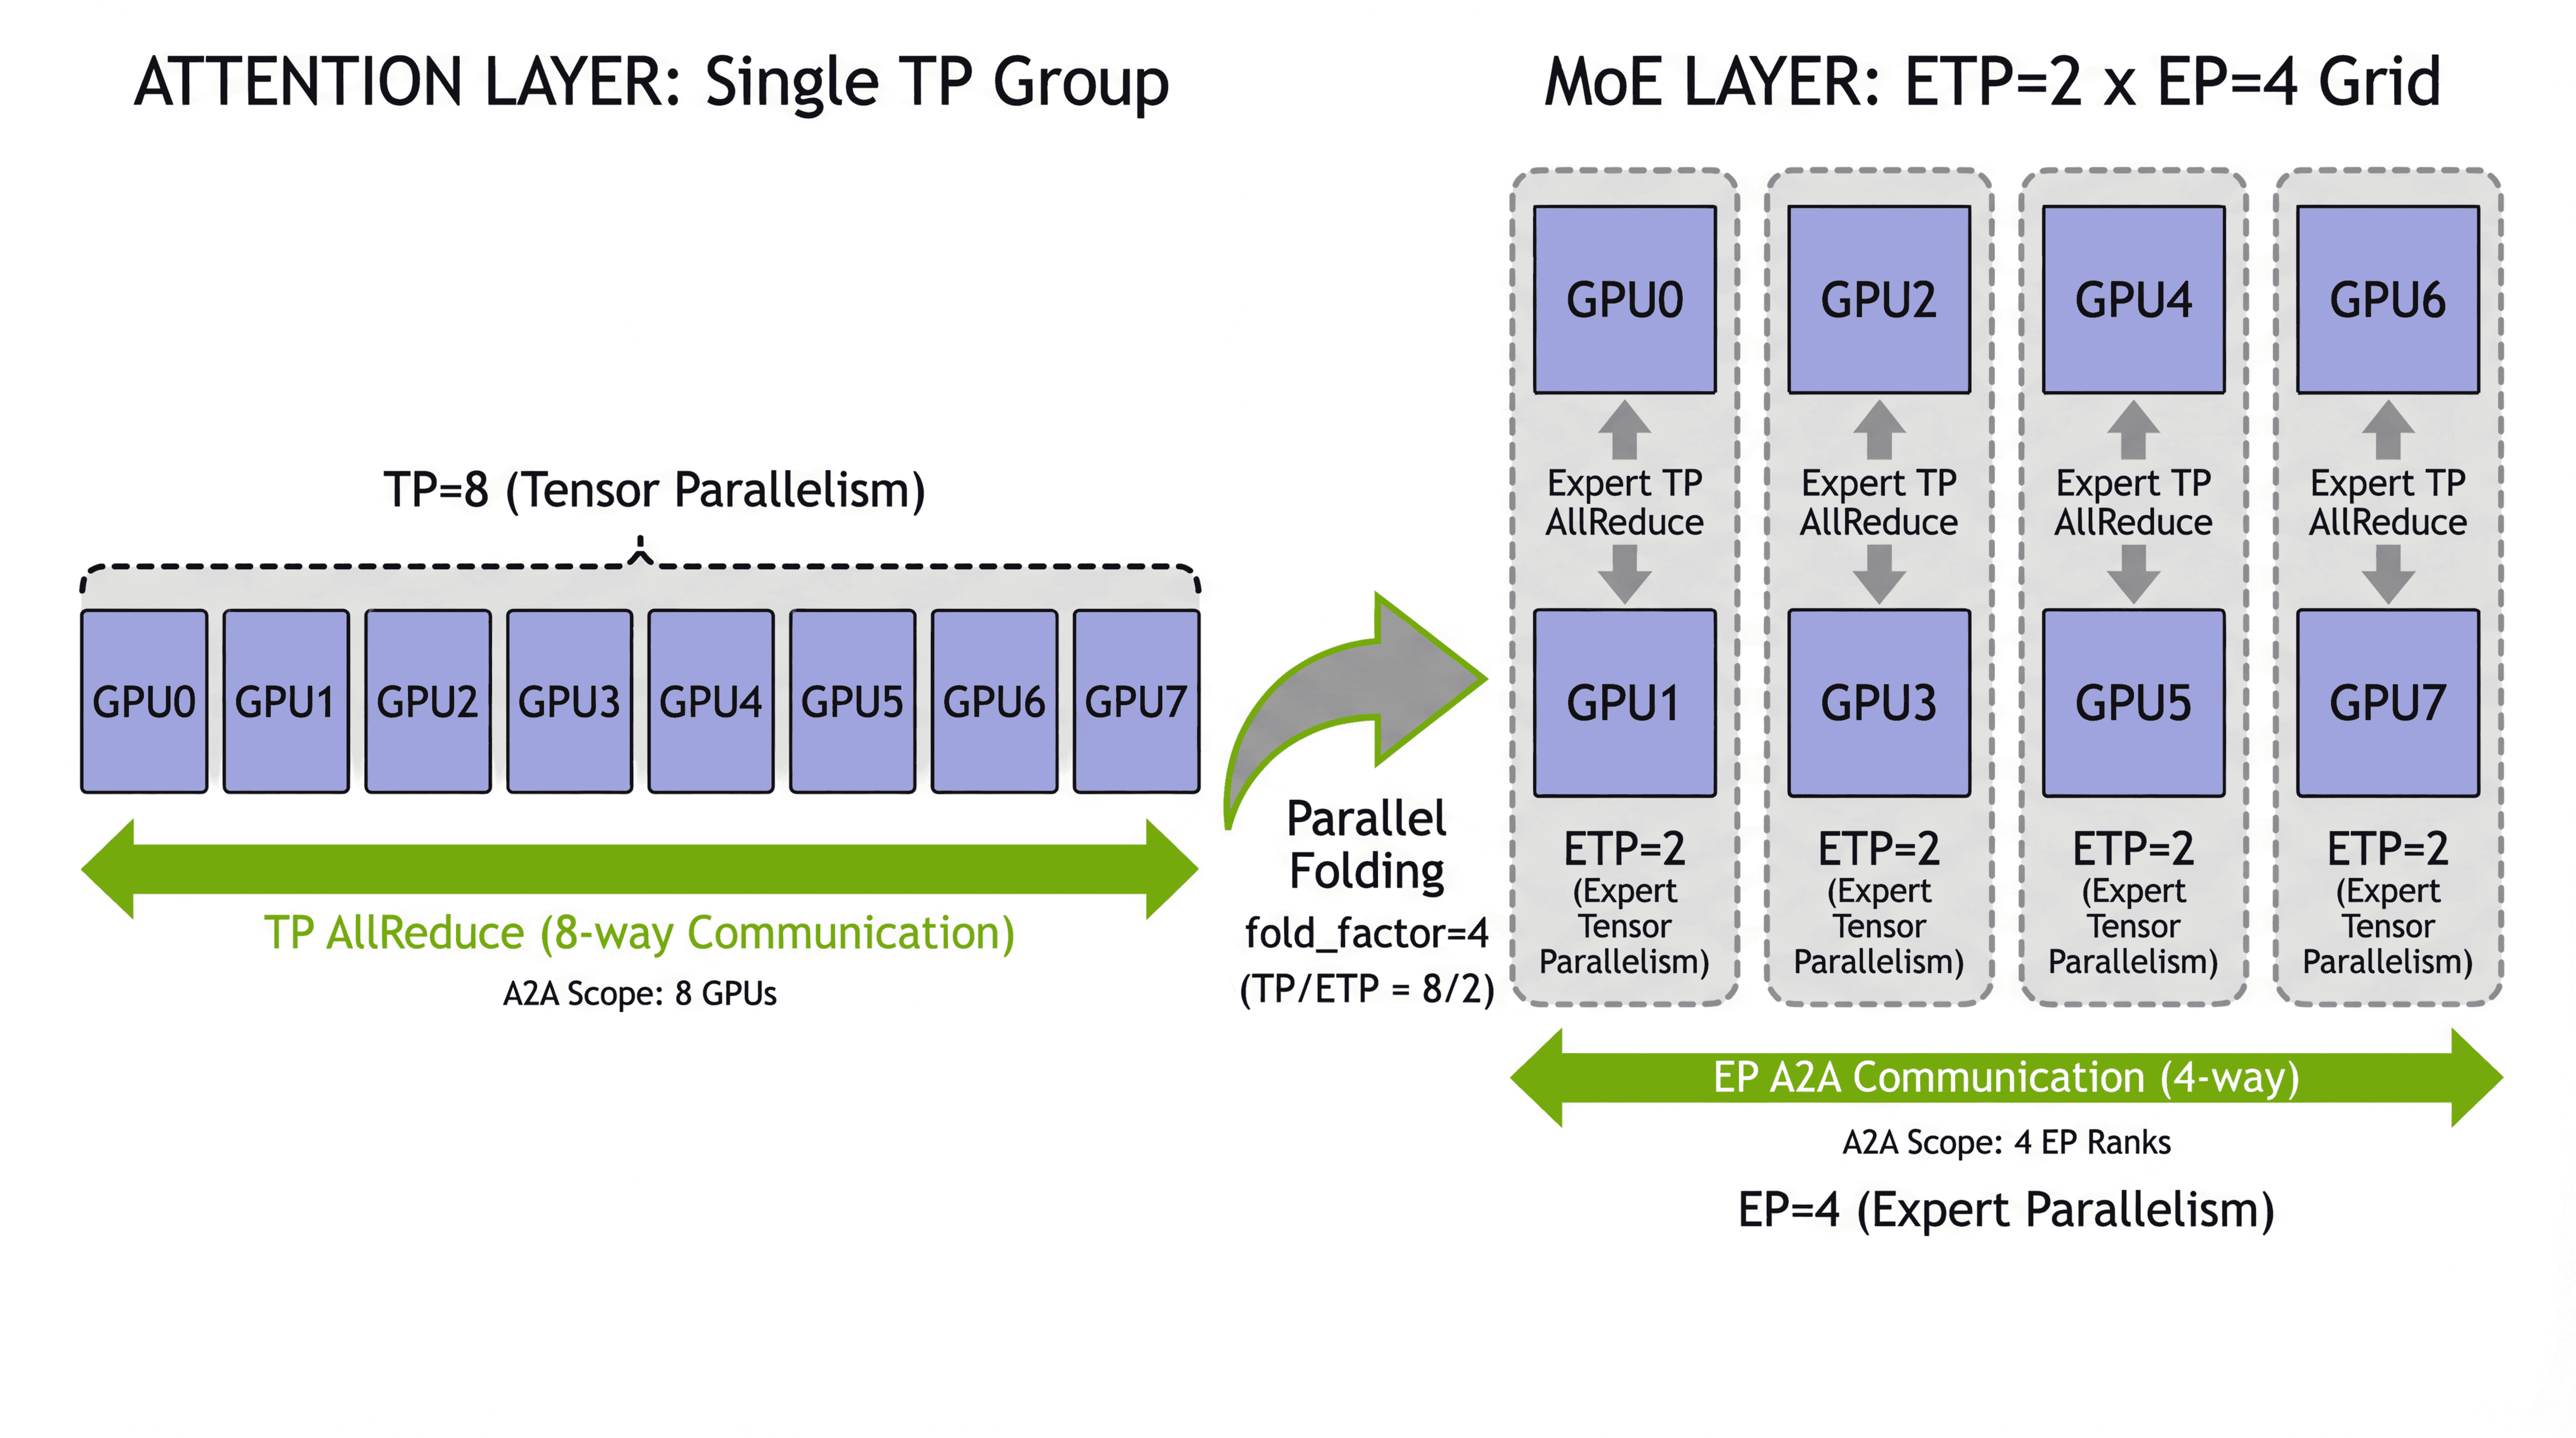
\includegraphics[width=0.9\textwidth]{figures/plots/parallel_folding_detailed_draft.png}
    \caption{并行折叠：解耦注意力和 MoE 并行映射。}
    \label{fig:parallel-folding-detailed}
\end{figure}

\subsubsection{概括}

本节讨论了 \emph{分销挑战} 用于教育部培训。核心问题是 \emph{稠密-稀疏失配}，根源于 MoE 的稀疏性：注意力层和 MoE 层具有冲突的最佳并行配置，但先前的框架迫使它们共享一种配置。 \textbf{MoE平行折叠} 通过解耦并行映射来解决这个问题，允许注意力使用高 TP/CP，而 MoE 独立使用高 EP。 Megatron-Core 与分布式优化器和 FSDP 一起将所有并行维度编排到一个统一框架中，将 MoE 训练扩展到数千个 GPU。

然而，仅可扩展的分布并不能保证训练效率。第~节中确定的三个基本障碍\ref{sec:challenges}内存、通信和计算效率墙仍然必须解决。以下部分介绍了威震天核心突破这些墙壁的解决方案。

\section{扩展 MoE：打破内存、通信和计算效率壁垒}\label{key-features-optimizations}

部分~\ref{parallelism-strategies} 已确立的 \emph{如何} 在数千个 GPU 上分配 MoE 训练。本节地址 \emph{如何提高效率}。挑战是巨大的：节~\ref{sec:challenges} 确定了由 MoE 稀疏驱动的参数计算不匹配而出现的三个基本障碍（内存墙、通信墙和计算效率墙）。这些墙不仅带来不便，而且还带来了麻烦。如果不解决这些问题，训练大规模 MoE 模型要么不可行（内存），要么速度极慢（通信、计算）。

\textbf{为什么是这三堵墙？} 这些障碍来自 GPU 加速训练的基本资源：内存存储参数和激活、互连在设备之间传输数据以及计算单元执行操作。每个训练系统都必须获得足够的内存，将数据移动到需要的地方，并有效地执行计算。其他潜在的瓶颈，例如用于检查点或主机端数据加载的存储 I/O，也存在，但运行的时间尺度允许它们与训练迭代重叠。三堵墙代表了每次前后传递的严格限制。

\textbf{墙壁相互作用。} 这些挑战并不是独立的；它们形成了一个紧密耦合的系统，修复一堵墙可能会暴露或恶化另一堵墙。考虑一个具体的优化轨迹：训练 1000B MoE 模型的团队首先遇到内存墙：仅激活就超过了 GPU 容量。它们启用激活重新计算（第~\ref{sec:memory-wall}），通过在向后传递过程中重新生成激活来交换内存以进行计算。内存限制得到解决，分析显示现在全面通信占据主导地位；计算墙隐藏了通信墙。他们实现了通信-计算重叠（第~\ref{sec:comm-wall}），通过专家执行来管道化所有到所有的传输。但细粒度专家的完成速度比沟通速度快，从而限制了重叠效率。它们可以实现降低精度的训练（第~\ref{sec:reduced-precision-training}）以减少内存占用，允许更大的批处理大小，从而提供更多的计算来隐藏通信。这是可行的，但引入了量化内核，它会分割执行流并增加内核启动开销。系统变为主机绑定：GPU 在内核启动之间空闲。他们部署 CUDA 图形（部分~\ref{sec:compute-wall}）以减少启动开销，但图需要静态张量形状，这与无丢包路由的动态专家分配相冲突。每个解决方案都会在系统中产生涟漪，要求同时了解所有三堵墙。孤立地解决墙壁问题会导致解决方案次优；有效的优化需要将内存、通信和计算视为一个统一的系统。

Megatron-Core 通过集成系统设计解决了这些挑战。本节的其余部分介绍了按其主要解决的墙组织的解决方案：
\begin{itemize}
    \item \textbf{部分~\ref{sec:memory-wall}：打破记忆墙。} 我们如何在 GPU 内存限制内适应训练？本节涵盖激活管理、重新计算策略、卸载和分布式参数存储。
    \item \textbf{部分~\ref{sec:comm-wall}：打破沟通壁垒。} 我们如何最大限度地减少设备间通信损失的时间？本节涵盖优化调度程序、通信计算重叠和管道集成。
    \item \textbf{部分~\ref{sec:compute-wall}：打破计算效率壁垒。} 我们如何保持 GPU 的工作饱和度？本节介绍内核融合、CUDA 图和无滴 MoE 的无同步执行。
\end{itemize}

FP8/FP4 中的降低精度训练可同时在所有三堵墙上提供优势，在第 1 节中单独介绍~\ref{sec:reduced-precision-training}。长上下文 MoE 训练会在注意力主导计算时改变优化平衡，在第 5 节中进行了讨论~\ref{sec:long-context-training}.

\subsection{打破记忆墙}\label{sec:memory-wall}

内存是 MoE 训练中的第一个硬约束：如果参数、优化器状态和激活的组合占用空间超过 GPU 容量，则训练无法继续。随着模型和专家数量的增长，内存需求快速增长，这使得内存优化对于实际训练至关重要。理解 \emph{在哪里} 内存消耗对于有效的优化至关重要。

\subsubsection{内存剖析：内存消耗的来源}

由于几个不同的开销来源，MoE 模型通常比同等的密集模型消耗更多的内存。考虑使用 BF16 精度训练的 DeepSeek-V3 $\text{PP}4 \times \text{VPP}4 \times \text{EP}64$ 跨 256 个 GPU 的配置。表~\ref{tab:memory-breakdown} 显示了每个 GPU 内存细分，显示总需求为 199.5 GB，远远超出未经优化的 H100 GPU 的 80 GB 容量。

\begin{table}[ht]
\centering
\caption{使用 BF16 训练的 DeepSeek-V3 每个 GPU 的内存细分（$\text{PP}4 \times \text{VPP}4 \times \text{EP}64$，256 个 GPU）。}
\label{tab:memory-breakdown}
\begin{tabular}{lrl}
\toprule
\textbf{成分} & \textbf{每个 GPU 的内存} & \textbf{优化技术} \\
\midrule
重量 \& 渐变 & 36.4GB & PP、EP 或 TP 分片 \\
主要重量 \& 优化器状态 & 32.1GB & 分布式优化器，BF16矩 \\
激活 & 131.0GB & 低精度、重新计算、卸载 \\
\midrule
\textbf{全部的} & \textbf{199.5GB} & \\
\bottomrule
\end{tabular}
\end{table}

三个组成部分促成了这一足迹：

\textbf{权重和梯度 (36.4 GB)。} 全部 $E$ 专家参数必须保留在内存中，即使只有 $K$ 激活每个令牌。 DeepSeek-V3 具有 top-8 路由的 256 个专家说明了这一点：685B 个参数，但每个令牌仅激活 37B，即 18 个$\times$ 差距。

\textbf{优化器状态 (32.1 GB)。} Adam 存储每个参数的动量和方差，使 FP32 中的参数内存增加三倍。使用 BF16 矩的混合精度训练减少了这种开销，但并没有消除它。

\textbf{激活 (131.0 GB)。} 最大的内存消耗，超过了权重和优化器状态的总和。 MoE 激活随着层深度、隐藏维度和顶部而缩放$k$，以及批量大小和序列长度。这使得激活成为主要优化目标。

\begin{notebox}
在大规模 MoE 训练中，激活主导着内存消耗，通常超过权重、梯度和优化器状态的组合内存。这使得激活内存优化成为实现更大批量或更灵活并行配置的最高优先级。
\end{notebox}

其他 MoE 特定因素会增加内存压力：动态路由可能会造成负载不平衡，某些专家会暂时收到太多令牌，并且通常必须填充令牌以适应高效的计算内核，从而消耗超出实际数据的内存。这些是激活内存成本，可以通过下面讨论的重新计算技术来降低。 ECHO 进一步解决了负载不平衡问题（第~\ref{sec:echo}），动态克隆热门专家以平衡不同级别的代币分配。

无法通过更改模型架构来减少内存，因此优化必须针对数据的存储和管理方式。四种互补策略可解决内存限制：

\begin{enumerate}
    \item \textbf{降低存储精度。} 较低精度的格式（FP8/FP4 而不是 BF16）可减少激活内存，同时对精度的影响最小。内存高效排列完全消除了冗余的中间张量。
    \item \textbf{用计算换取存储。} 激活重新计算 \cite{chen2016training,korthikanti2022reducingactivationrecomputationlarge,beaumont2021optimal} 在前向传递过程中丢弃中间结果，并在向后传递过程中重新生成它们，以计算周期换取内存容量。
    \item \textbf{卸载到主机内存。} 当 GPU 内存耗尽时，激活可以在前向传递期间传输到 CPU 内存，并在后向传递期间检索，用 PCIe 带宽换取 GPU 内存 \cite{ren2021zerooffload}.
    \item \textbf{跨设备分发。} 完全分片数据并行 (FSDP) \cite{zhao2023pytorchfsdp,rajbhandari2020zero,rajbhandari2021zeroinf,rajbhandari2023zeropp} 跨数据并行等级划分参数、梯度和优化器状态，​​从而能够训练超出单设备容量的模型。 
\end{enumerate}

以下小节将这些技术分为两组。首先，按开销排序的激活内存优化：零开销（内存高效排列）、精度权衡（FP8/FP4 与 BF16）、计算权衡（重新计算）和带宽权衡（卸载）。然后，针对权重和优化器状态的优化：精度感知优化器和分配策略（FSDP）。

\subsubsection{内存高效排列：零开销激活减少}\label{sec:mem-eff-permute}

最理想的内存优化是那些没有计算开销的优化。内存高效排列通过简单的代数重排消除冗余的中间张量来实现这一点。该技术是零开销的，因为它只是改变 \emph{什么时候} 应用路由器概率，而不是 \emph{无论} 它们被应用；在传统的实现方式中，向后传递所需的预激活缓冲区无论如何都会被存储。

正如章节中所描述的~\ref{sec:moe-layer-architecture}，路由器将每个令牌分配给其顶部$k$ 具有学习路由权重的专家，并且加权专家输出被组合以产生最终结果。

考虑一个令牌 $\mathbf{x}$ 路由到其顶部-$k$ 专家。让 $\mathcal{T}(\mathbf{x}) \subset \{1,\dots,E\}$ 用路由权重表示选定的专家集 $\{p_i\}_{i \in \mathcal{T}(\mathbf{x})}$。各位专家 $E_i$ 是一个带有权重矩阵的两层 MLP $\mathbf{W}_1^{(i)}, \mathbf{W}_2^{(i)}$ 和非线性激活 $\phi$ （例如，SwiGLU）：
\[
E_i(\mathbf{x}) = \mathbf{W}_2^{(i)}\,\phi\!\bigl(\mathbf{W}_1^{(i)}\mathbf{x}\bigr).
\]
在 \textbf{标准制定}，应用路由权重 \emph{后} 专家计算：
\begin{equation}\label{eq:moe-standard-combine}
\mathbf{y} = \sum_{i \in \mathcal{T}(\mathbf{x})} p_i \cdot \mathbf{W}_2^{(i)}\,\phi\!\bigl(\mathbf{W}_1^{(i)}\mathbf{x}\bigr).
\end{equation}
\textbf{内存高效排列} 吸收 $p_i$ 进入激活状态，应用它 \emph{前} 第二个线性层：
\begin{equation}\label{eq:moe-mem-eff-combine}
\mathbf{y} = \sum_{i \in \mathcal{T}(\mathbf{x})} \mathbf{W}_2^{(i)}\,\bigl(p_i \cdot \phi\!\bigl(\mathbf{W}_1^{(i)}\mathbf{x}\bigr)\bigr).
\end{equation}
当专家没有偏见条件时， $\mathbf{W}_2^{(i)}$ 是纯线性映射和标量乘法交换： $p_i \cdot \mathbf{W}_2^{(i)}\mathbf{h} = \mathbf{W}_2^{(i)}(p_i \cdot \mathbf{h})$ 对于任意向量 $\mathbf{h}$， 所以 \eqref{eq:moe-standard-combine} 和 \eqref{eq:moe-mem-eff-combine} 在数学上是等价的。


\begin{figure}[ht]
    \centering
    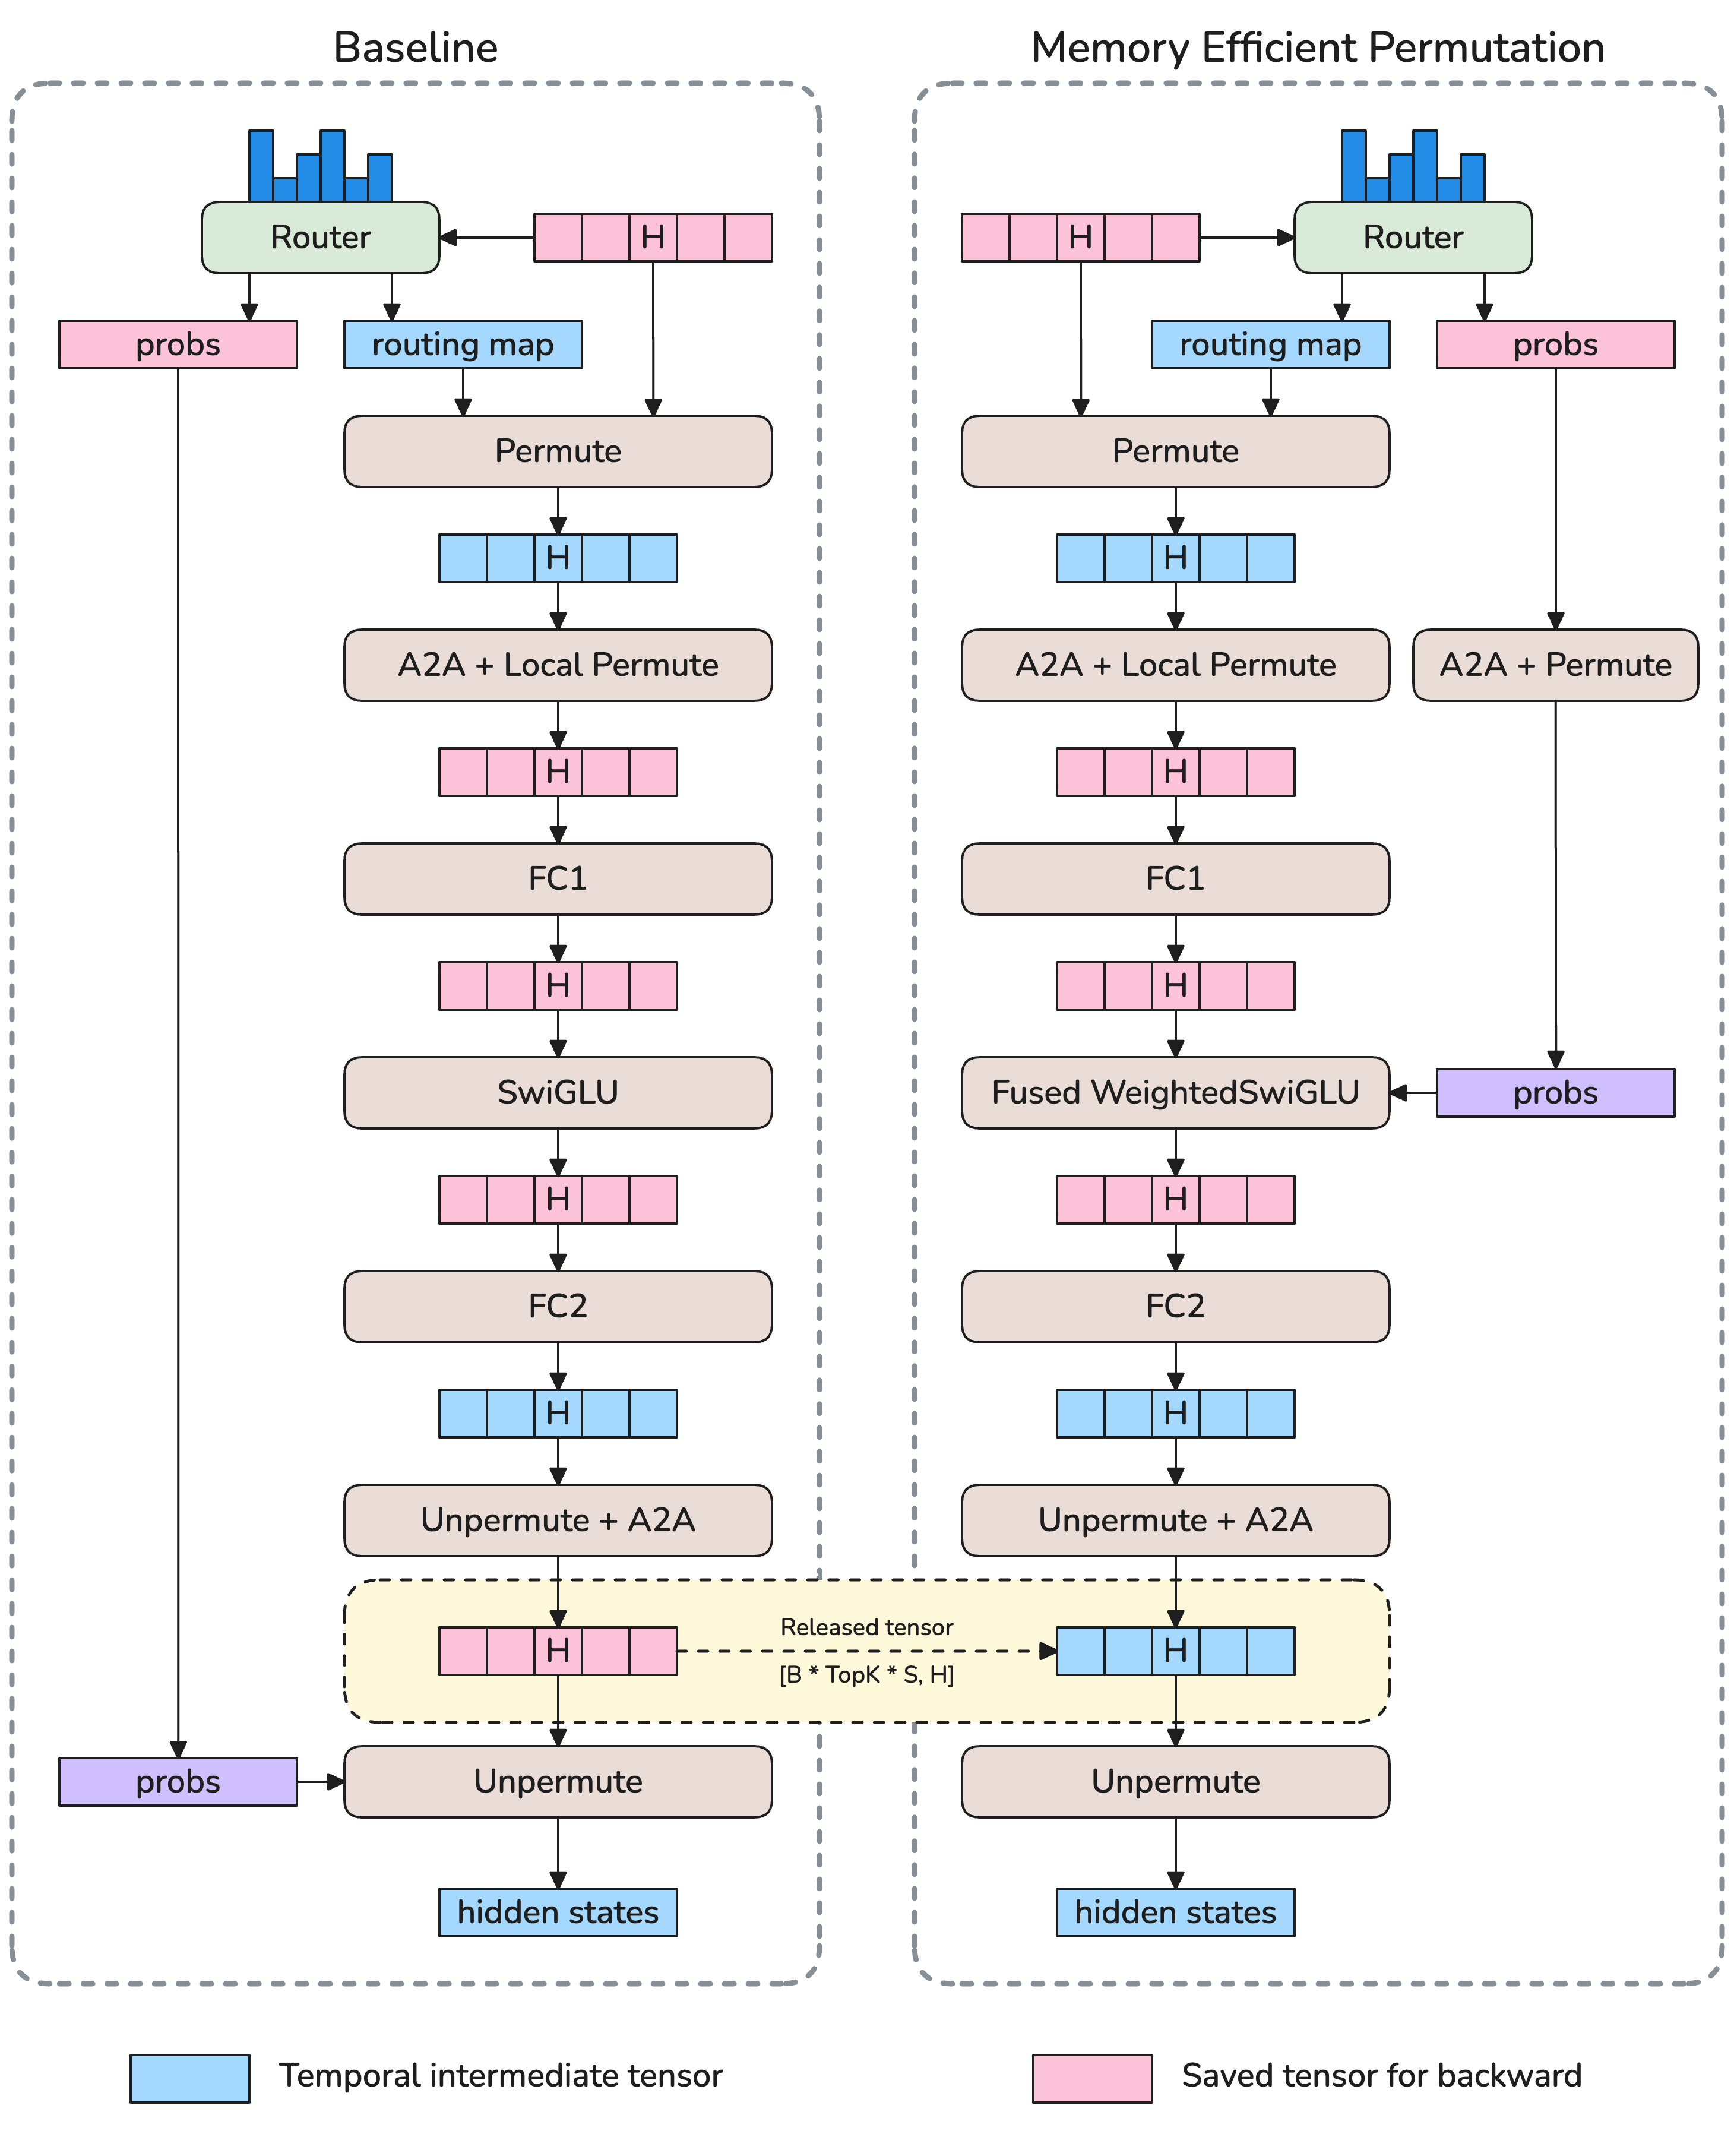
\includegraphics[width=0.6\linewidth]{figures/memory_efficient_permutation.png}
        \caption{内存高效排列。}
    \label{fig:mem-eff-permute}
\end{figure}

这种重新排列通过消除路由器向后传递所需的已保存张量来减少峰值内存。让 $\mathbf{z}_i = \mathbf{W}_1^{(i)}\mathbf{x}$ 表示预激活输入。在标准制定中，计算 $\partial \mathcal{L}/\partial p_i$ 需要保留每个专家的输出 $E_i(\mathbf{x})$ 整个向后传球。在内存效率公式中， $p_i$ 乘以 $\phi(\mathbf{z}_i)$ 直接，所以 $\partial \mathcal{L}/\partial p_i$ 仅取决于 $\phi(\mathbf{z}_i)$，融合后向内核重新计算 $\mathbf{z}_i$ 在飞行中。自从 $\mathbf{z}_i$ 无论是否使用内存高效排列，都必须已保存用于 SwiGLU 激活自身的后向传递，不会引入额外的缓冲区，从而在零计算开销的情况下产生峰值内存的净减少。 \Figref{fig:mem-eff-permute} 说明了这种转变。

对于 DeepSeek-V3（表~\ref{tab:memory-breakdown}），内存高效排列为每个 GPU 节省了大约 26.3 GB 的激活内存，显着减少且计算成本为零。

\subsubsection{降低精度训练：用于减少激活内存的 FP8/FP4}\label{sec:fp8-activation}

将激活存储在 FP8/FP4 而不是 BF16 中可以减少内存占用，同时对模型质量的影响最小。

在前向传递过程中，必须保留每个线性层的输入，以计算后向传递中的权重梯度。在 Transformer 模型中，这些线性层输入构成了大部分激活记忆：注意力投影（Q、K、V、输出）和 MLP 层（包括 MoE 中的专家 MLP）各自保存其输入以进行梯度计算。通过将这些输入张量存储在 FP8/FP4 而不是 BF16 中，每个张量的内存占用量减少了 50\%/75\%。

表中为DeepSeek-V3配置~\ref{tab:memory-breakdown}，启用 FP8 训练可减少大约 16 GB 的激活内存，相当于大约 12\% 131 GB 激活预算。这相当于将适合 FP8 存储的约 32 GB 线性层输入减半。其余的激活（注意力分数、标准化中间值、路由张量）要么需要更高的精度以实现数值稳定性，要么不跨前向-后向边界存储。这种减少与其他激活优化（例如重新计算和卸载）正交，允许将它们组合起来以实现累积节省。

\textit{有关降低精度训练机制的详细信息，包括配方、量化策略和 MoE 特定的优化，请参阅第~\ref{sec:reduced-precision-training}.}

\subsubsection{重新计算：用计算换取内存}\label{sec:recomputation}

激活重新计算（或激活检查点）是一种成熟的技术，它在前向传递期间丢弃中间激活并在向后传递期间重新计算它们 \cite{chen2016training}。然而，简单的全层重新计算可以添加 $\sim$33\% 计算开销，对于 MoE 层来说成本更高，因为重新计算专家计算也会重新触发 EP 的全对全通信。威震天核心介绍 \textit{细粒度的} 仅针对内存最密集但计算成本最低的操作进行重新计算，以最小的开销实现显着的内存节省 \cite{korthikanti2022reducingactivationrecomputationlarge}。

两种技术组成了该策略（\figref{fig:selective-recomputation}):

\begin{figure}[ht]
    \centering
    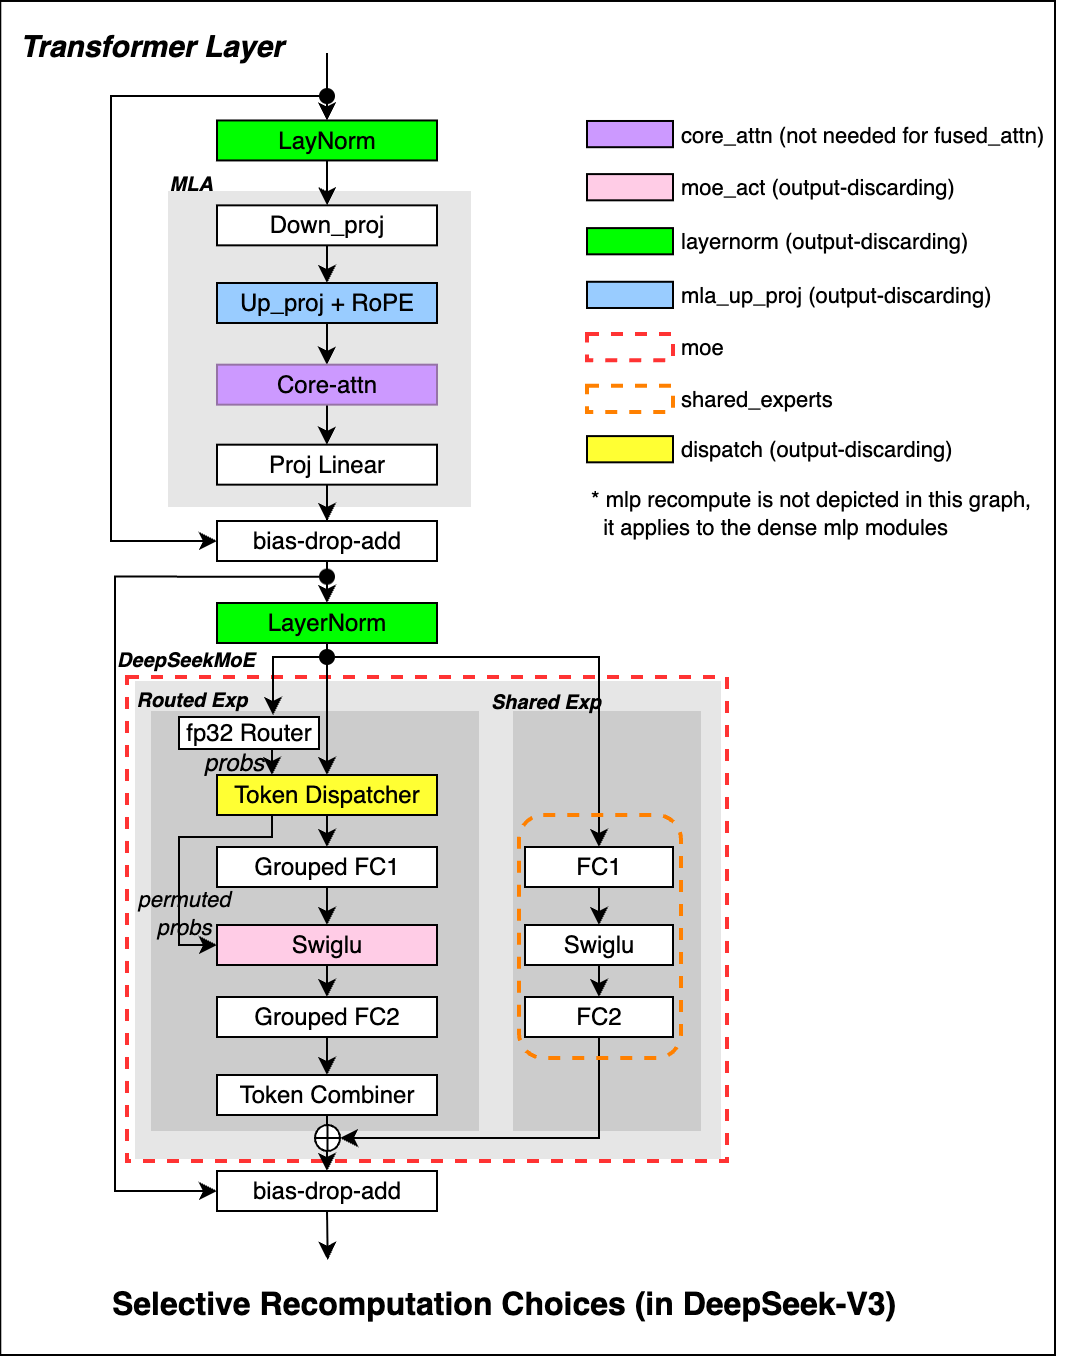
\includegraphics[width=0.5\linewidth]{figures/selective-recomputation.png}
        \caption{选择性重新计算。}
    \label{fig:selective-recomputation}
\end{figure}

\textbf{粒度重新计算。} 用户不是将激活检查点应用于大型整体部分，而是准确指定在向后传递中重新计算哪些计算。例如，可以仅重新计算专家 MLP 中的激活函数、LayerNorm 模块或多重潜在注意力 (MLA) 中的上投影。通过重新计算单个操作或子模块，只需适度增加计算工作量即可实现显着的内存节省，因为只有选定的部分需要重新计算（少于 5\% 额外的计算开销）。

\textbf{输出丢弃重新计算。} 传统的激活检查点工作流程将检查点模块的输出传递到下游层，存储这些输出以供反向传播使用。然而，由于这些输出将在向后传递期间重新计算，因此该存储是多余的。为了避免这种情况，Megatron-Core MoE 在被后续层消耗后立即释放检查点模块的输出。在向后传递期间，从重新计算的结果恢复输出。该策略确保不会为可以廉价恢复的激活保留不必要的内存，从而在不影响梯度正确性或训练动态的情况下减少内存占用。

表~\ref{tab:recomputation-savings} 表中总结了 DeepSeek-V3 配置的不同重新计算目标所实现的内存减少~\ref{tab:memory-breakdown}.

\begin{table}[ht]
\centering
\caption{通过 DeepSeek-V3 的细粒度重新计算减少每个 GPU 的内存（$\text{PP}4 \times \text{VPP}4 \times \text{EP}64$，256 个 GPU）。}
\label{tab:recomputation-savings}
\begin{tabular}{lr}
\toprule
\textbf{重新计算目标} & \textbf{每个 GPU 节省的内存} \\
\midrule
MLA 上投影 & 30.4GB \\
激活函数 (SwiGLU) & 3.8GB \\
层规范 & 8.2GB \\
\midrule
\textbf{全部的} & \textbf{42.4GB} \\
\bottomrule
\end{tabular}
\end{table}

\subsubsection{细粒度激活卸载}\label{sec:offloading}

% \footnote{This is collaborative work between NVIDIA and Rednote.} the footnote has been removed
当精度和重新计算优化后 GPU 内存仍然不足时， \textit{卸载} 激活 CPU 内存可提供额外的容量。与以计算周期换取内存的重新计算不同，卸载以 PCIe 带宽为代价。挑战在于隐藏计算背后的传输延迟，以便卸载看起来“免费”。

\paragraph{动机}
细粒度的 MoE 模型具有极端的参数膨胀：DeepSeek-V3 每个代币仅激活 37B（18$\times$ 比例，表~\ref{tab:memory-breakdown}）； Kimi-K2 总计达到 1T，其中 32B 处于活动状态（31$\times$）。这个参数计算不匹配（小节~\ref{sec:challenges}) 对于卸载尤其严重，因为激活内存不会随着专家并行 (EP) 或管道并行 (PP) 的增加而减少；这些策略减少了参数记忆，而不是激活记忆。

Transformer Engine 提供层级卸载，但这种粗粒度限制了有效性。层内的不同模块具有显着不同的内存与计算比率：LayerNorm 激活很小且重新计算成本低廉，而 \texttt{expert\_fc1} 输入很大但计算成本很高。层级卸载无法区分这些情况。它要么卸载所有内容（浪费带宽），要么什么也不卸载（浪费内存）。

\paragraph{高级思想：重叠和预取。}
GPU 的复制引擎和计算引擎独立运行。当模块的计算时间超过其激活传输时间时，D2H副本可以零成本与后续计算同时运行。 \Figref{fig:activation-offloading-timeline} 说明了前向和后向传递的流重叠机制。

\begin{figure}[ht]
    \centering
    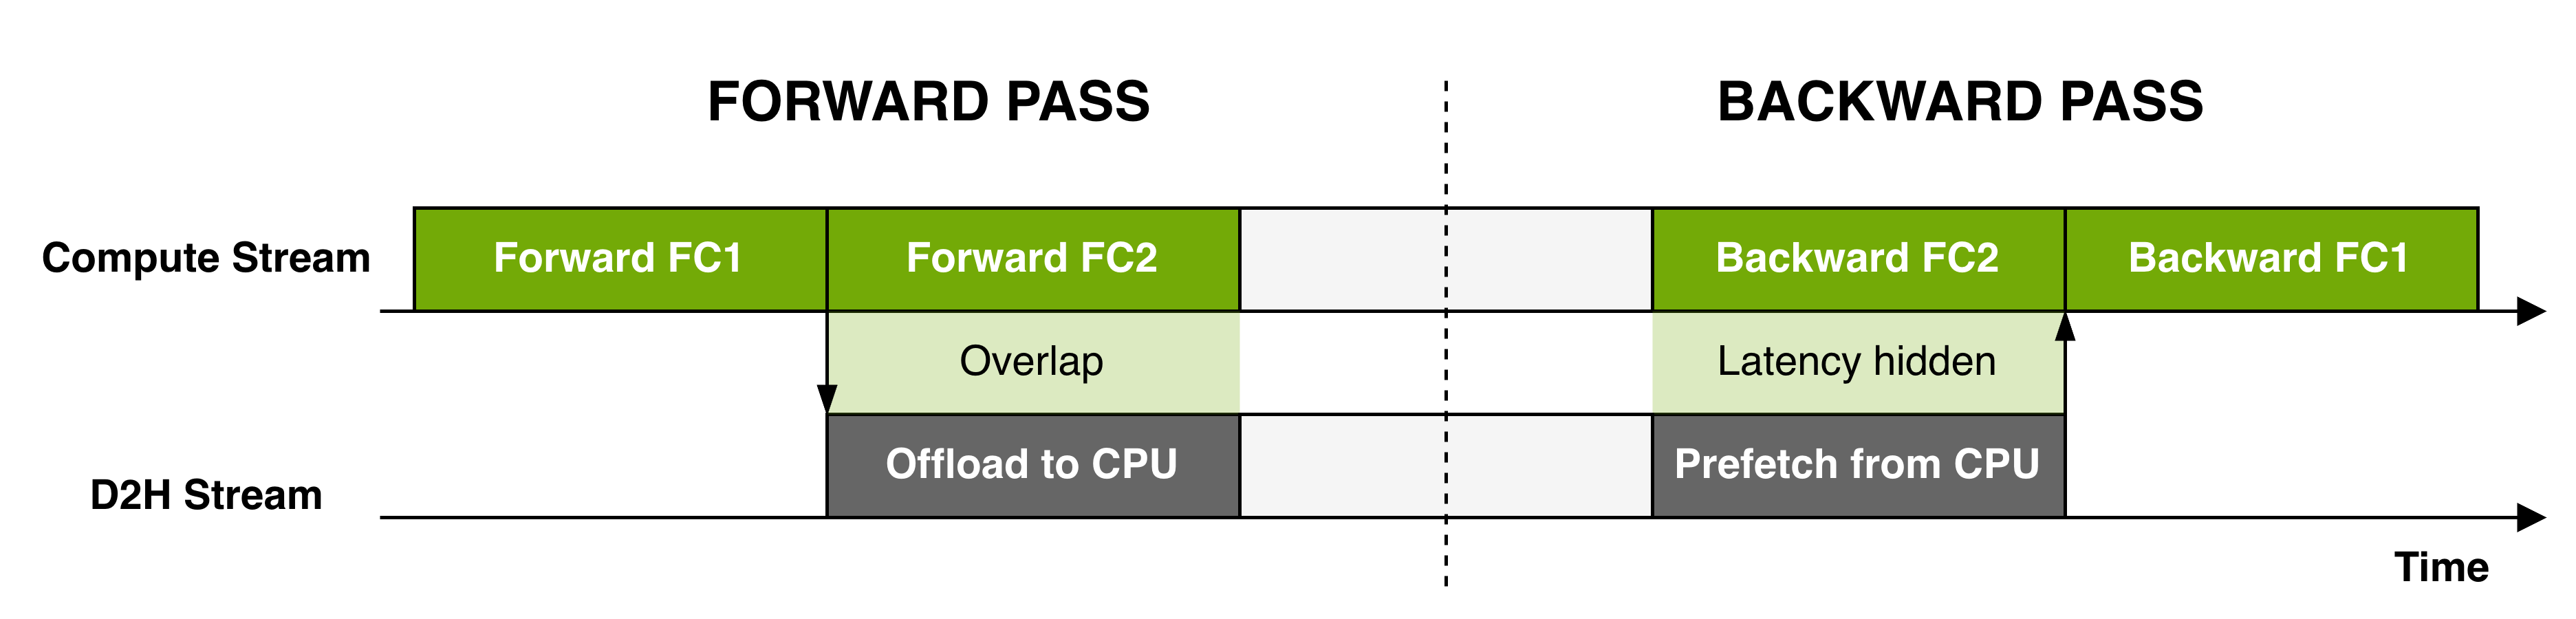
\includegraphics[width=0.9\textwidth]{figures/activation_offloading_timeline.drawio.png}
    \caption{细粒度激活卸载：前向和后向传递的流重叠。}
    \label{fig:activation-offloading-timeline}
\end{figure}

\paragraph{向前传球。}
在前向传播期间，输入激活在模块计算后立即卸载到 CPU，通过专用 D2H 流与下一个模块的计算并行运行。一个例外：最后一层的激活不会被卸载，因为在后向过程中立即需要它们，因此没有计算可用于隐藏传输延迟。

\paragraph{向后传球。}
在反向传播期间，激活重新加载遵循 \textit{层交错重载} 模式：系统重新加载同一模块的激活（例如， \texttt{expert\_fc1}）从 \textit{下一个} 层，同时计算当前层的梯度。发生重新加载 \textit{后} 每个模块都向后完成，因此每个模块类型在任何时候只有一个激活驻留在 GPU 内存中，从而避免了双倍激活存储的需要。当单个模块具有非常大的激活（其中 2$\times$ 内存占用会导致意外的内存峰值。

\paragraph{PP 和 VPP 处理。}
对于PP/VPP场景， \texttt{Chunk\-Offload\-Handler} 管理每个（微批次、VPP 阶段）组合的卸载/重新加载逻辑，与 PP=1 情况相同。主要挑战是管理虚拟管道块之间的数据依赖性和执行顺序。处理程序按倒序 (FILO) 排列到双端队列中，并按正序 (FIFO) 排列微批次。在向后过程中，弹出的处理程序会自动匹配 VPP 块执行顺序，从而将卸载的激活与其相应的向后传递正确配对。

\paragraph{主要技术特点。}
\begin{itemize}[itemsep=2pt,topsep=4pt]
    \item \textbf{模块级粒度：} 用户指定通过哪些模块卸载 \verb|--offload-modules|，启用混合策略。轻量级模块（LayerNorm、激活）使用重新计算，而昂贵的模块（注意、专家）则使用卸载。
    \item \textbf{异步传输：} 专用 D2H/H2D CUDA 流与计算并行运行传输； CUDA 事件仅在必要时协调同步。
    \item \textbf{重新计算积分：} 与细粒度重新计算相结合（\secref{sec:recomputation}）。为了 \texttt{moe\_act}，两种策略都适用：重新计算激活，同时卸载其输入，释放整个 \texttt{fc1}$\rightarrow$\texttt{act} 链。
    \item \textbf{CUDA 图形兼容性：} 使用外部事件而不是流同步，允许通过 CUDA 图形外部的计算隐藏卸载模块。
    \item \textbf{全场景兼容：} 支持PP=1/PP$>$1/VPP$>$1、所有精度（BF16/FP8/MXFP8/NVFP4）、具有全对全重叠的 1F1B 和 MoE/MLA 架构。
\end{itemize}

\paragraph{相对于完全重新计算的峰值内存优势。}
完整的重新计算存储每一层的 \textit{输入} 在 GPU 上，同时释放中间激活；向后根据这些存储的输入重新计算中间值。对于一个 $L$-层模型，GPU峰值显存为 $L \times \text{layer\_input} + 1 \times \text{layer\_intermediate}$。相反，卸载将层输入移至 CPU；在后退期间，每个输入在使用前重新加载并在使用后立即释放。这可将 GPU 峰值内存减少至 $1 \times \text{layer\_input} + 1 \times \text{layer\_intermediate}$，与模型深度无关。对于深度模型（例如 60 多个层），这代表了完全重新计算无法实现的基本内存优势。

\paragraph{表现。}
细粒度卸载和重新计算作为互补策略一起工作（\figref{fig:offloading-recomputation}）：像 LayerNorm 这样的轻量级操作使用重新计算，而像注意力和专家这样昂贵的模块则使用卸载。异步传输与计算重叠以隐藏 PCIe 延迟。表~\ref{tab:offloading-results} 显示多种配置的结果。细粒度卸载减少内存10--18\% 仅1.6--2\% 吞吐量开销。在训练Qwen3-235B的情况下，卸载可以降低张量并行度，这 \textit{改善} 吞吐量提高 15.0\% 具有几乎相同的内存成本。

\begin{table}[ht]
\centering
\caption{细粒度激活卸载对内存和吞吐量的影响。}
\label{tab:offloading-results}
\begin{tabular}{lccccc}
\toprule
\textbf{模型 \& 配置} & \textbf{基线} & \textbf{+卸载} & \textbf{内存 $\Delta$} & \textbf{吞吐量 $\Delta$} \\
\midrule
DeepSeek-V3完整版 & 169GB & 151GB & $-$10.7\% & $-$1.6\% \\
{\small TP1PP8EP32VPP4、MXFP8} & 945TF/秒 & 930TF/秒 & & \\
\midrule
Qwen3-235B  & 172GB & 175GB & $+$1.7\% & $+$15.0\% \\
{\small TP2$\rightarrow$TP1+EP16$\rightarrow$EP64} & 800 TF/秒 & 920TF/秒 & & \\
\bottomrule
\end{tabular}
\end{table}

\begin{figure}[ht]
    \centering
    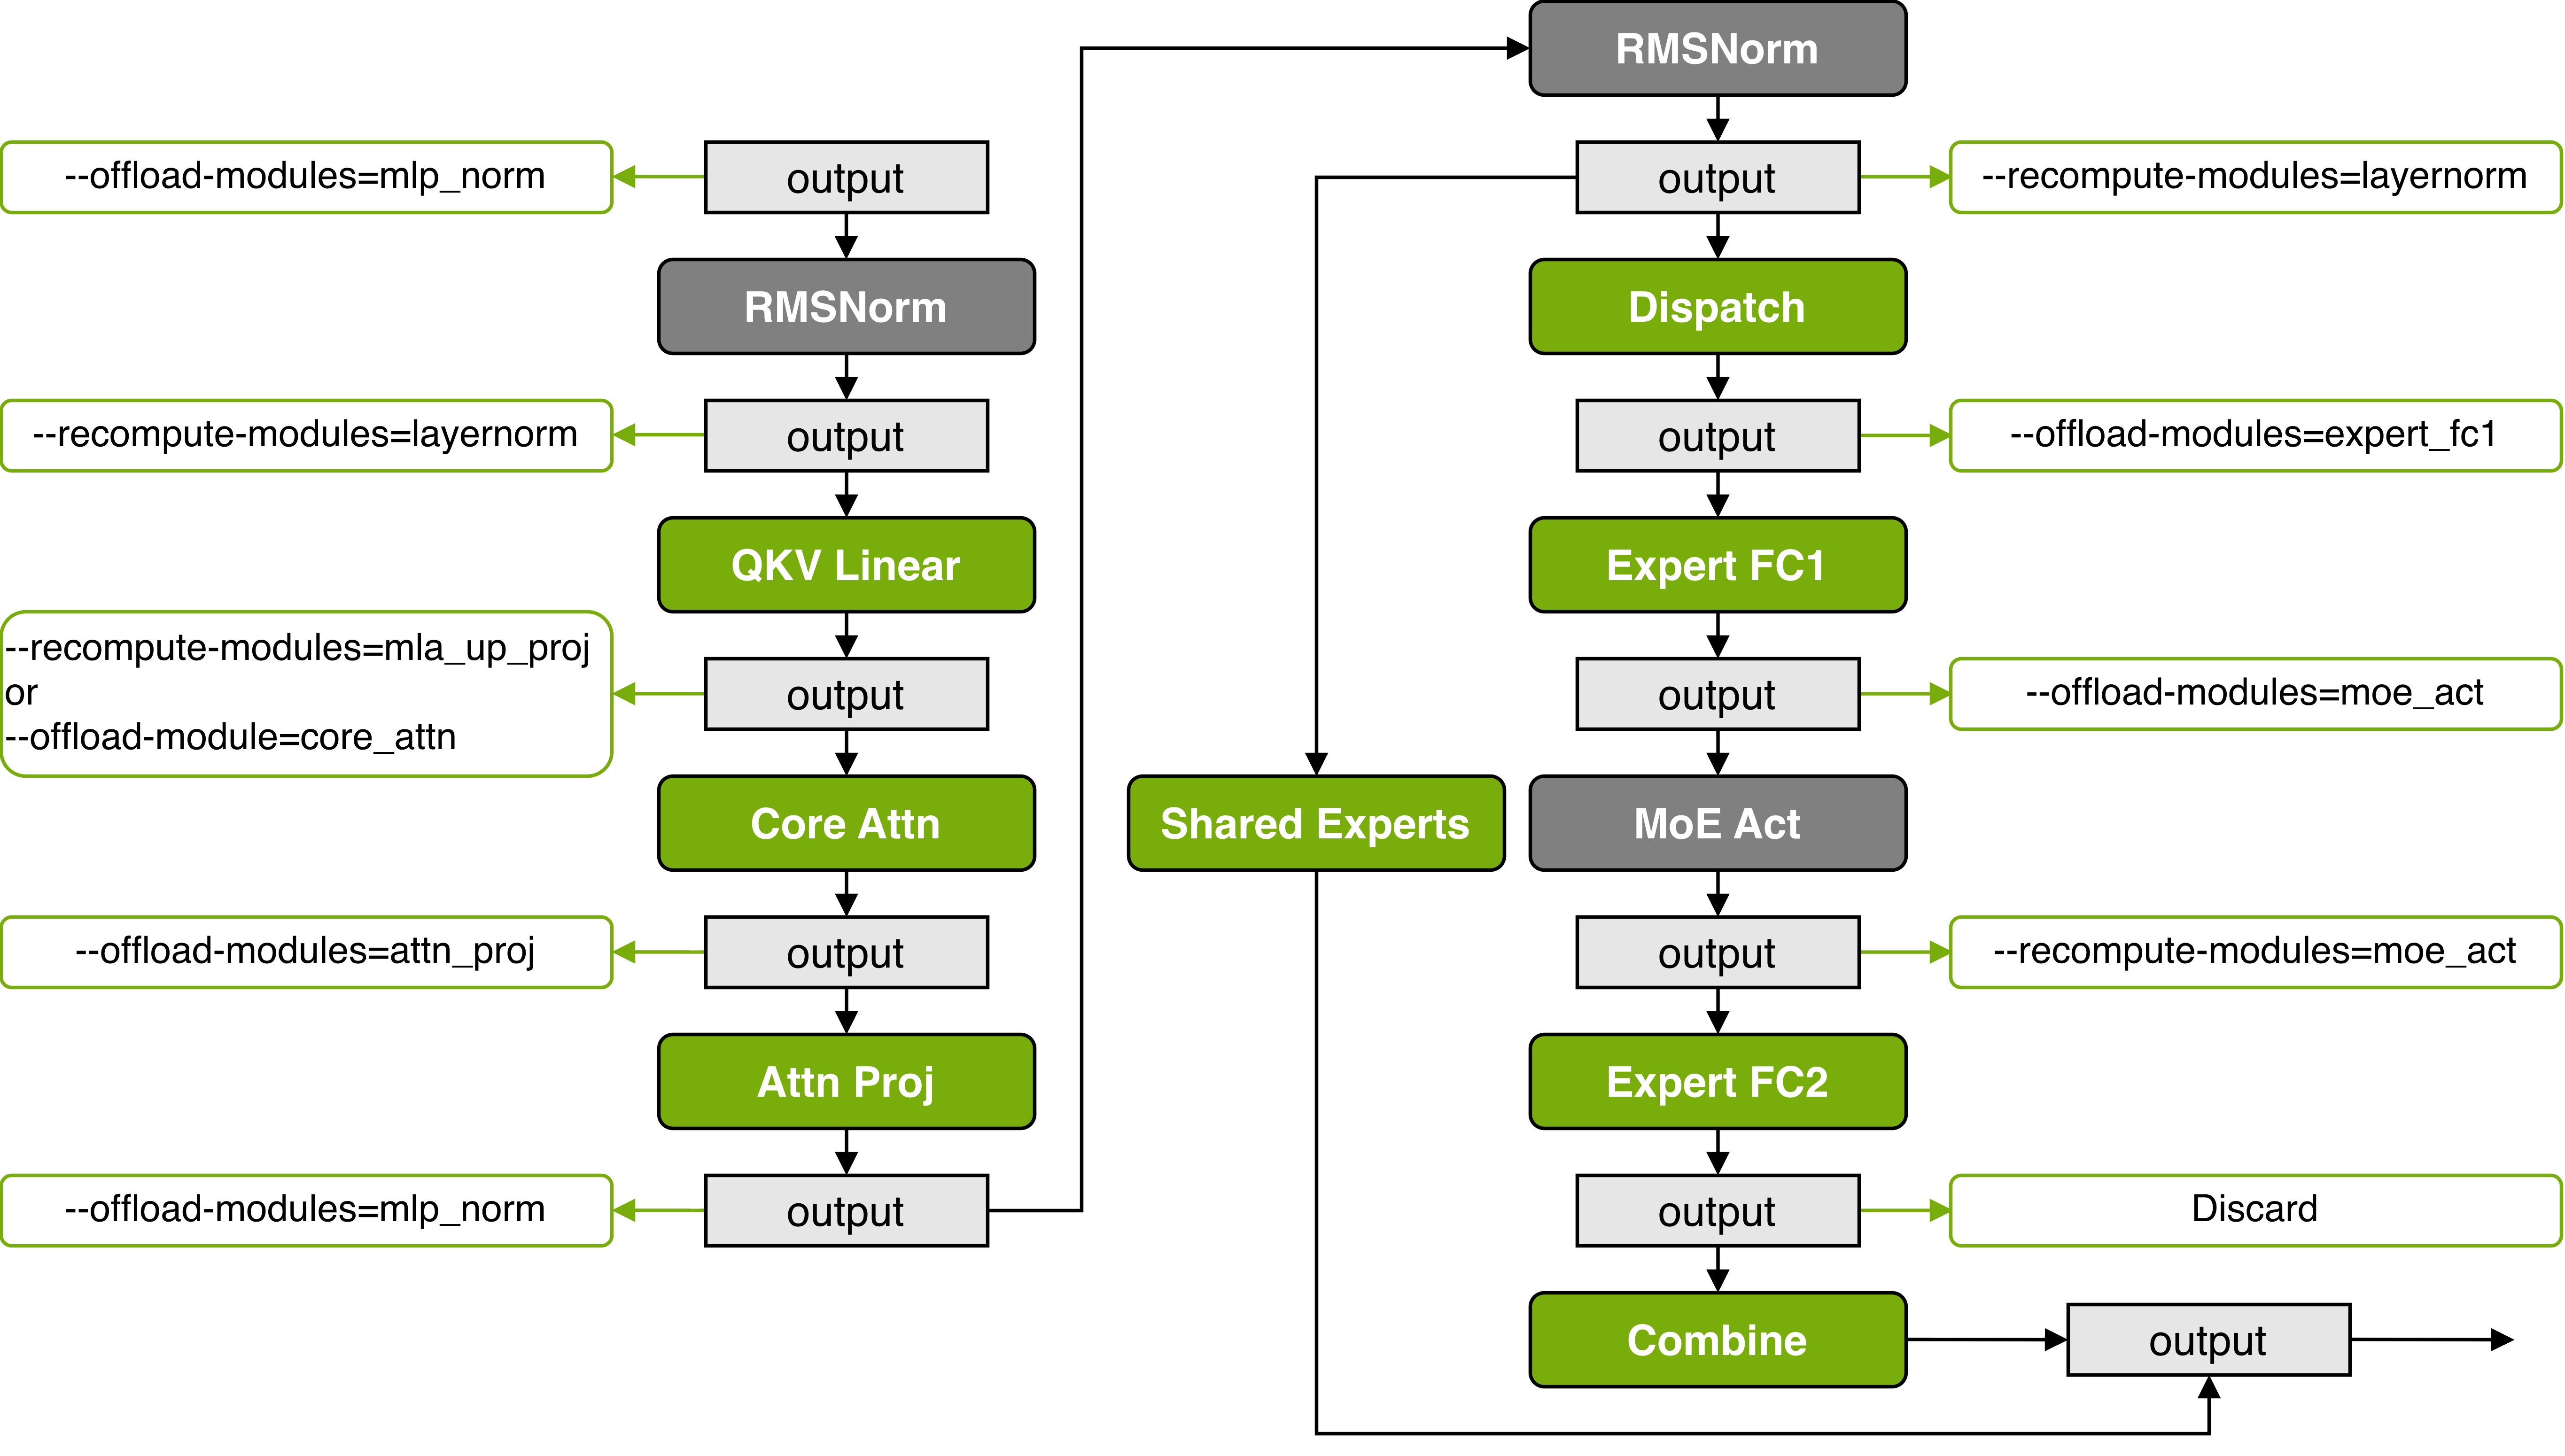
\includegraphics[width=0.8\linewidth]{figures/offloading_recomputation.png}
    \caption{细粒度卸载和重新计算：互补的内存优化策略。}
    \label{fig:offloading-recomputation}
\end{figure}

\subsubsection{权重和优化器优化：低精度存储和卸载}\label{sec:precision-opt}

前面的优化针对的是激活内存，它在内存崩溃中占主导地位。不过表~\ref{tab:memory-breakdown} 显示主要权重和优化器状态每个 GPU 消耗 32.1 GB，相当于 16\% 总内存占用量。对于具有数千亿参数的模型，该组件成为重要的优化目标。 Megatron-Core 提供两种技术：降低存储需求的精确感知优化，以及将非活动状态移出 GPU 的 CPU 卸载。

\paragraph{精度感知优化器。}
Adam 优化器 \cite{kingma2014adam} 每个参数维护两个状态张量：一阶矩 (\texttt{exp\_avg}) 和二阶矩 (\texttt{exp\_avg\_sq}）。传统实现将这些存储在 FP32 中，每个参数消耗 8 个字节，这对大规模训练造成了严重的内存瓶颈。关键的见解是，优化器状态可以容忍较低的存储精度而不影响收敛，前提是实际的更新计算保持较高的精度。

精度感知优化器将存储精度与计算精度解耦 \cite{dettmers2022optimizers8bit}。第一和第二时刻可以存储在 BF16（每个 2 个字节）甚至 FP8（每个 1 个字节）中，从而将每个参数的存储从 8 个字节减少到 4 个字节（BF16）或 2 个字节（FP8）。在每个优化器步骤中，这些低精度状态会在 TransformerEngine 的 FusedAdam 内核中动态转换为 FP32；更新是用全精度算术计算的，以保持数值稳定性。

该实现提供了四个可配置的精度级别：主梯度、主参数、一阶矩和二阶矩精度。在典型配置中，主要参数和梯度保留在 FP32 中以确保高质量的梯度更新，而矩估计则存储在 BF16 中 \cite{liu2024deepseek}。这实现了大约 50\% 减少优化器状态内存（与表中的 32.1 GB 预算相比，大约节省 10--12 GB）~\ref{tab:memory-breakdown}）对训练动态的影响可以忽略不计。

与分布式优化器结合使用时，它可以跨数据并行大小级别对优化器状态进行分片 $d$，每列的理论内存需求进一步降低。在使用 BF16 矩进行 DeepSeek-V3 训练时，每个 DP 等级每个参数的内存消耗从 $6+12/d$ 字节到 $6+8/d$ 字节。

\paragraph{状态卸载。}
在前向和后向传递期间，优化器状态占用 GPU 内存但保持不活动状态；卸载会回收该内存以用于其他操作。优化器状态卸载将优化器步骤保留在 GPU 上，但传输优化器状态（\texttt{exp\_avg}, \texttt{exp\_avg\_sq}）并在之后掌握CPU的权重 \texttt{optimizer.step()} 并在下一步之前重新加载它们。此方法使用 GPU 计算，同时在前向和后向传递过程中回收内存。

状态卸载对于具有高带宽互连的系统特别有效。在采用 NVLink-C2C 的 GB200 上，异步传输与计算重叠，固定内存可实现最大带宽利用率。对于 DeepSeek-V3，状态卸载可节省 15--20 GB GPU 内存 (47--62\% 32.1 GB 优化器和权重预算），每次迭代开销仅为 0.1--0.2 秒。

这两种技术提供了可以很好地协同工作的权衡。由于 FP32 转换发生在融合 Adam 内核中，因此精度感知优化器不会产生性能开销；它将优化器状态内存减少多达 50\%。 CPU 卸载可以节省更多内存（所有优化器状态和主权重），但会引入适度的传输开销。重要的是，这些技术组合得很好：使用具有 BF16 矩的精确感知存储可以减少必须卸载的状态大小，从而减少传输时间，并使卸载更加实用，即使在没有最高带宽互连的系统上也是如此。

\subsubsection{教育部 FSDP}\label{sec:fsdp-ref}

完全分片数据并行性 (FSDP) \cite{zhao2023pytorchfsdp,rajbhandari2020zero} 跨数据并行等级的分片模型参数、梯度和优化器状态，​​以便每个 GPU 仅保留一个本地分片。专家参数通常在 MoE 模型中占据主导地位，这使得 FSDP 成为专家并行性的自然补充。然而，两者必须正确组合。

\paragraph{为什么选择教育部的 FSDP？}

Megatron-FSDP 与多种并行策略无缝组合，包括专家并行 (EP)、张量并行 (TP) 和上下文并行 (CP)。对于大规模 MoE 模型，将 FSDP 与 EP 相结合，可以将 FSDP 的一般优势转化为专家繁重工作负载的具体优势。

\begin{itemize}[itemsep=2pt]
  \item \textbf{记忆力和沟通能力下降}：EP 为每个 GPU 分配一个专家子集，FSDP 将这些本地专家分片到专家数据并行 (EDP) 组而不是整个 DP 组。每 GPU 内存和集体体积均随 EDP 大小而不是总 DP 大小缩放，因此 MoE 模型可以在相同的硬件预算下支持更多专家或更大批量。

  \item \textbf{无 PP 灵活性}：FSDP+EP 避免了管道并行性的几个工程痛点，包括不均匀的 PP/VPP 阶段平衡、DeepSeek 式模型中输出和 MTP 层的放置以及多模态设置中的视觉编码器分区。配置减少到选择EP大小和FSDP分片程度，无需复杂的管道阶段设计。

  \item \textbf{广泛的型号兼容性}：Megatron-FSDP 支持两种模型实现路径：使用 Megatron-Core 自己的模块构建的模型和由标准组成的 PyTorch 原生模型 \texttt{torch.nn} 模块。两条路径都接收相同的 FSDP+EP 分片、通信优化和检查点支持。为了与 HuggingFace 生态系统实现互操作性，Megatron-Bridge 可以处理 HuggingFace 模型和 Megatron FSDP 之间的在线权重转换，因此用户可以加载预训练的 HuggingFace 检查点，使用 FSDP+EP 进行训练，然后将权重导出回来，而无需手动格式转换。
\end{itemize}

\paragraph{FSDP+EP：双DeviceMesh设计}

核心设计挑战是密集层和专家层需要不同的分片范围。密集模块（注意力、标准化）受益于整个 DP 组上的 FSDP 分片。 EP 首先对专家模块进行分区，因此每个 GPU 只保留其指定的专家。因此，FSDP 应在每个专家的数据并行 (EDP) 组内进行分片，而不是全局分片。

Megatron-FSDP 通过以下方法解决了这个问题 \emph{双设备网格} 建筑学。主 DeviceMesh 管理密集模块的 DP-Shard、DP-Outer、TP 和 CP。辅助 Expert DeviceMesh 通过 FSDP 管理 EP 模块，其范围仅限于 EDP 维度。每个变压器层自动将其子模块路由到适当的网格。注意力和标准化使用主网格，而 MoE 专家 FFN 层使用 Expert DeviceMesh。因此，专家参数的 AllGather 和 ReduceScatter 保留在小型 EDP 组内，而不是跨越所有 DP 等级。

% \begin{figure}[ht]
%     \centering
%     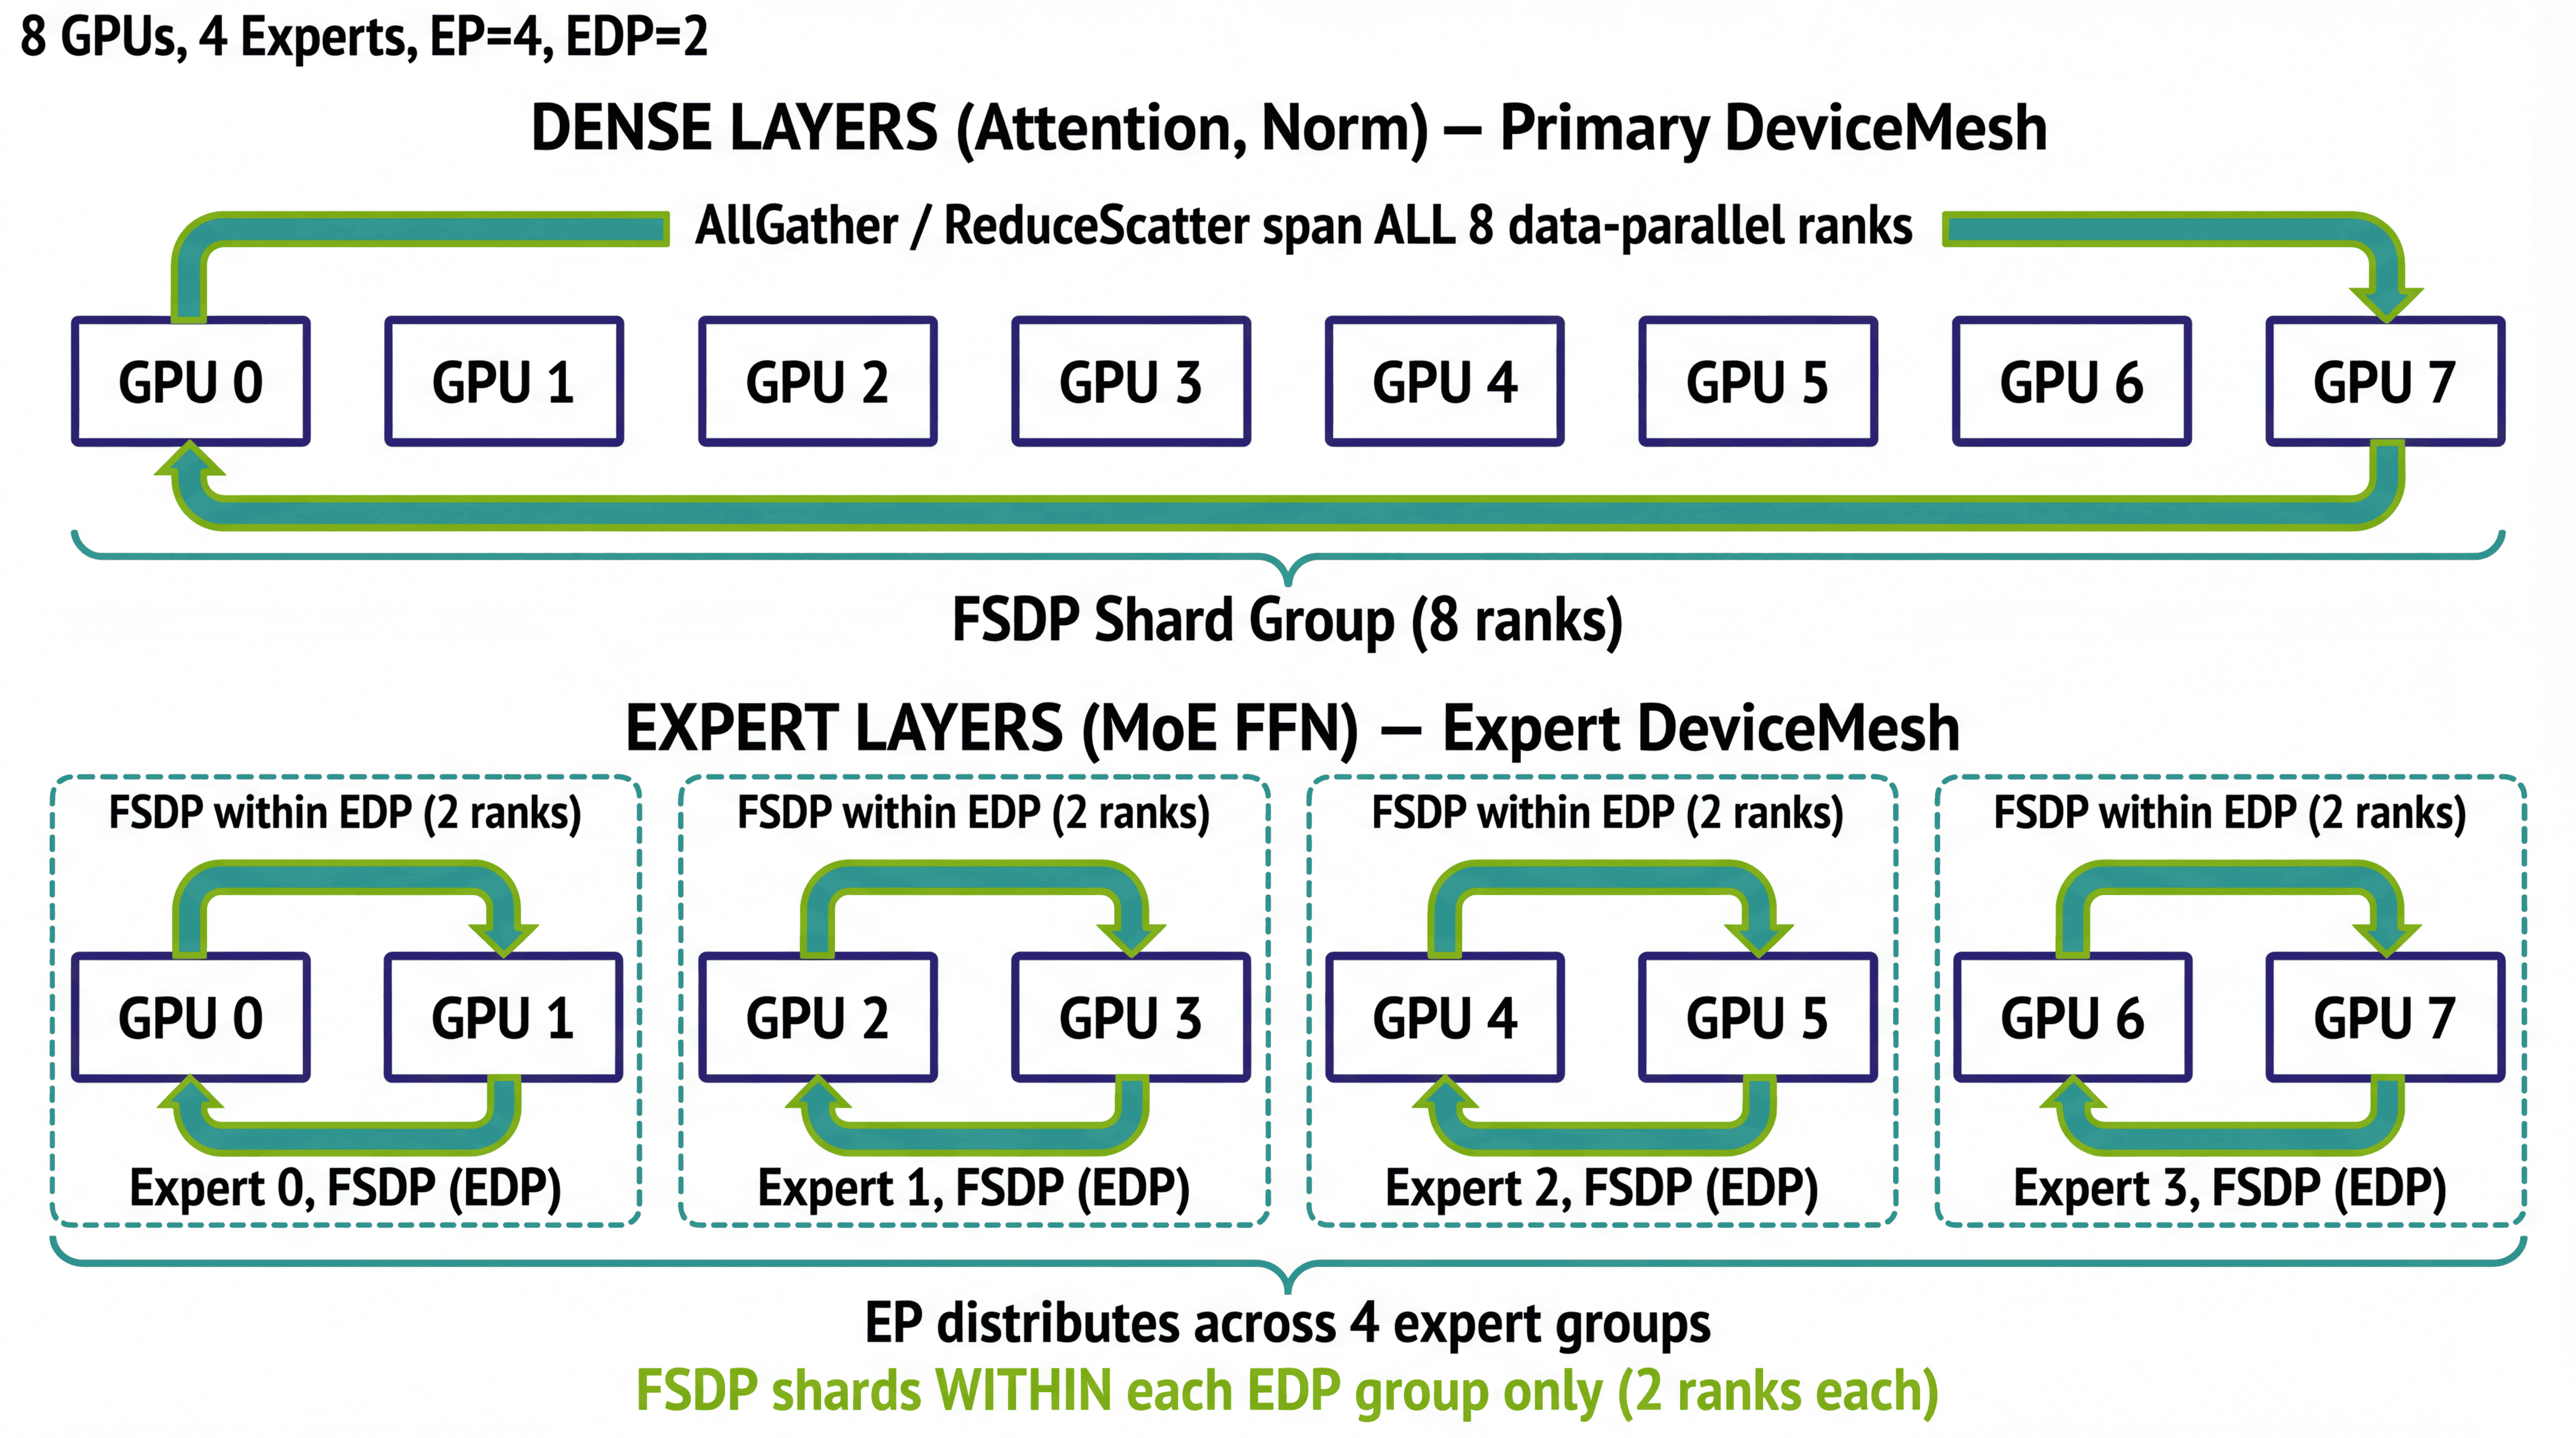
\includegraphics[width=0.95\textwidth]{figures/ai_gen/ai_gen_fsdp_ep_dual_devicemesh.png}
%     \caption{Dual DeviceMesh for FSDP+EP: primary mesh for dense layers, expert mesh for MoE layers.}
%     \label{fig:fsdp-ep-mesh}
% \end{figure}

对于大规模部署，此设计扩展到 \emph{混合分片数据并行} (HSDP)，添加外部 DP 复制维度。 HSDP 完全分片排名子集中的参数并跨子集复制，将 AllGather 限制在组内大小。双 DeviceMesh 为专家和非专家参数保留单独的外部 DP 组，利用 NVLink（节点内）和横向扩展互连（节点间）之间的带宽差距。

\paragraph{零拷贝通信}

双 DeviceMesh 确定哪些等级参与每个 FSDP 集体，但集体本身仍然会带来缓冲区管理和数据复制的开销。 Megatron-FSDP 通过两项优化消除了这种开销。

\textbf{1.非均匀分片：} 标准 FSDP2 沿其主维度独立地对每个参数进行分片，产生统一的每参数分片（图~\ref{fig:fsdp2-sharding}）。相反，Megatron-FSDP 会展平并连接模块内的所有参数，然后在设备之间应用非均匀分片（图~\ref{fig:mfsdp-sharding}）。然后，分片边界与通信缓冲区布局对齐，并且集合直接从扁平化存储中读取，无需冗余复制。在 Llama3 405B 训练中，这将通信开销减少了大约 10\%.

\begin{figure}[ht]
  \centering
  \begin{subfigure}[b]{0.45\textwidth}
    \centering
    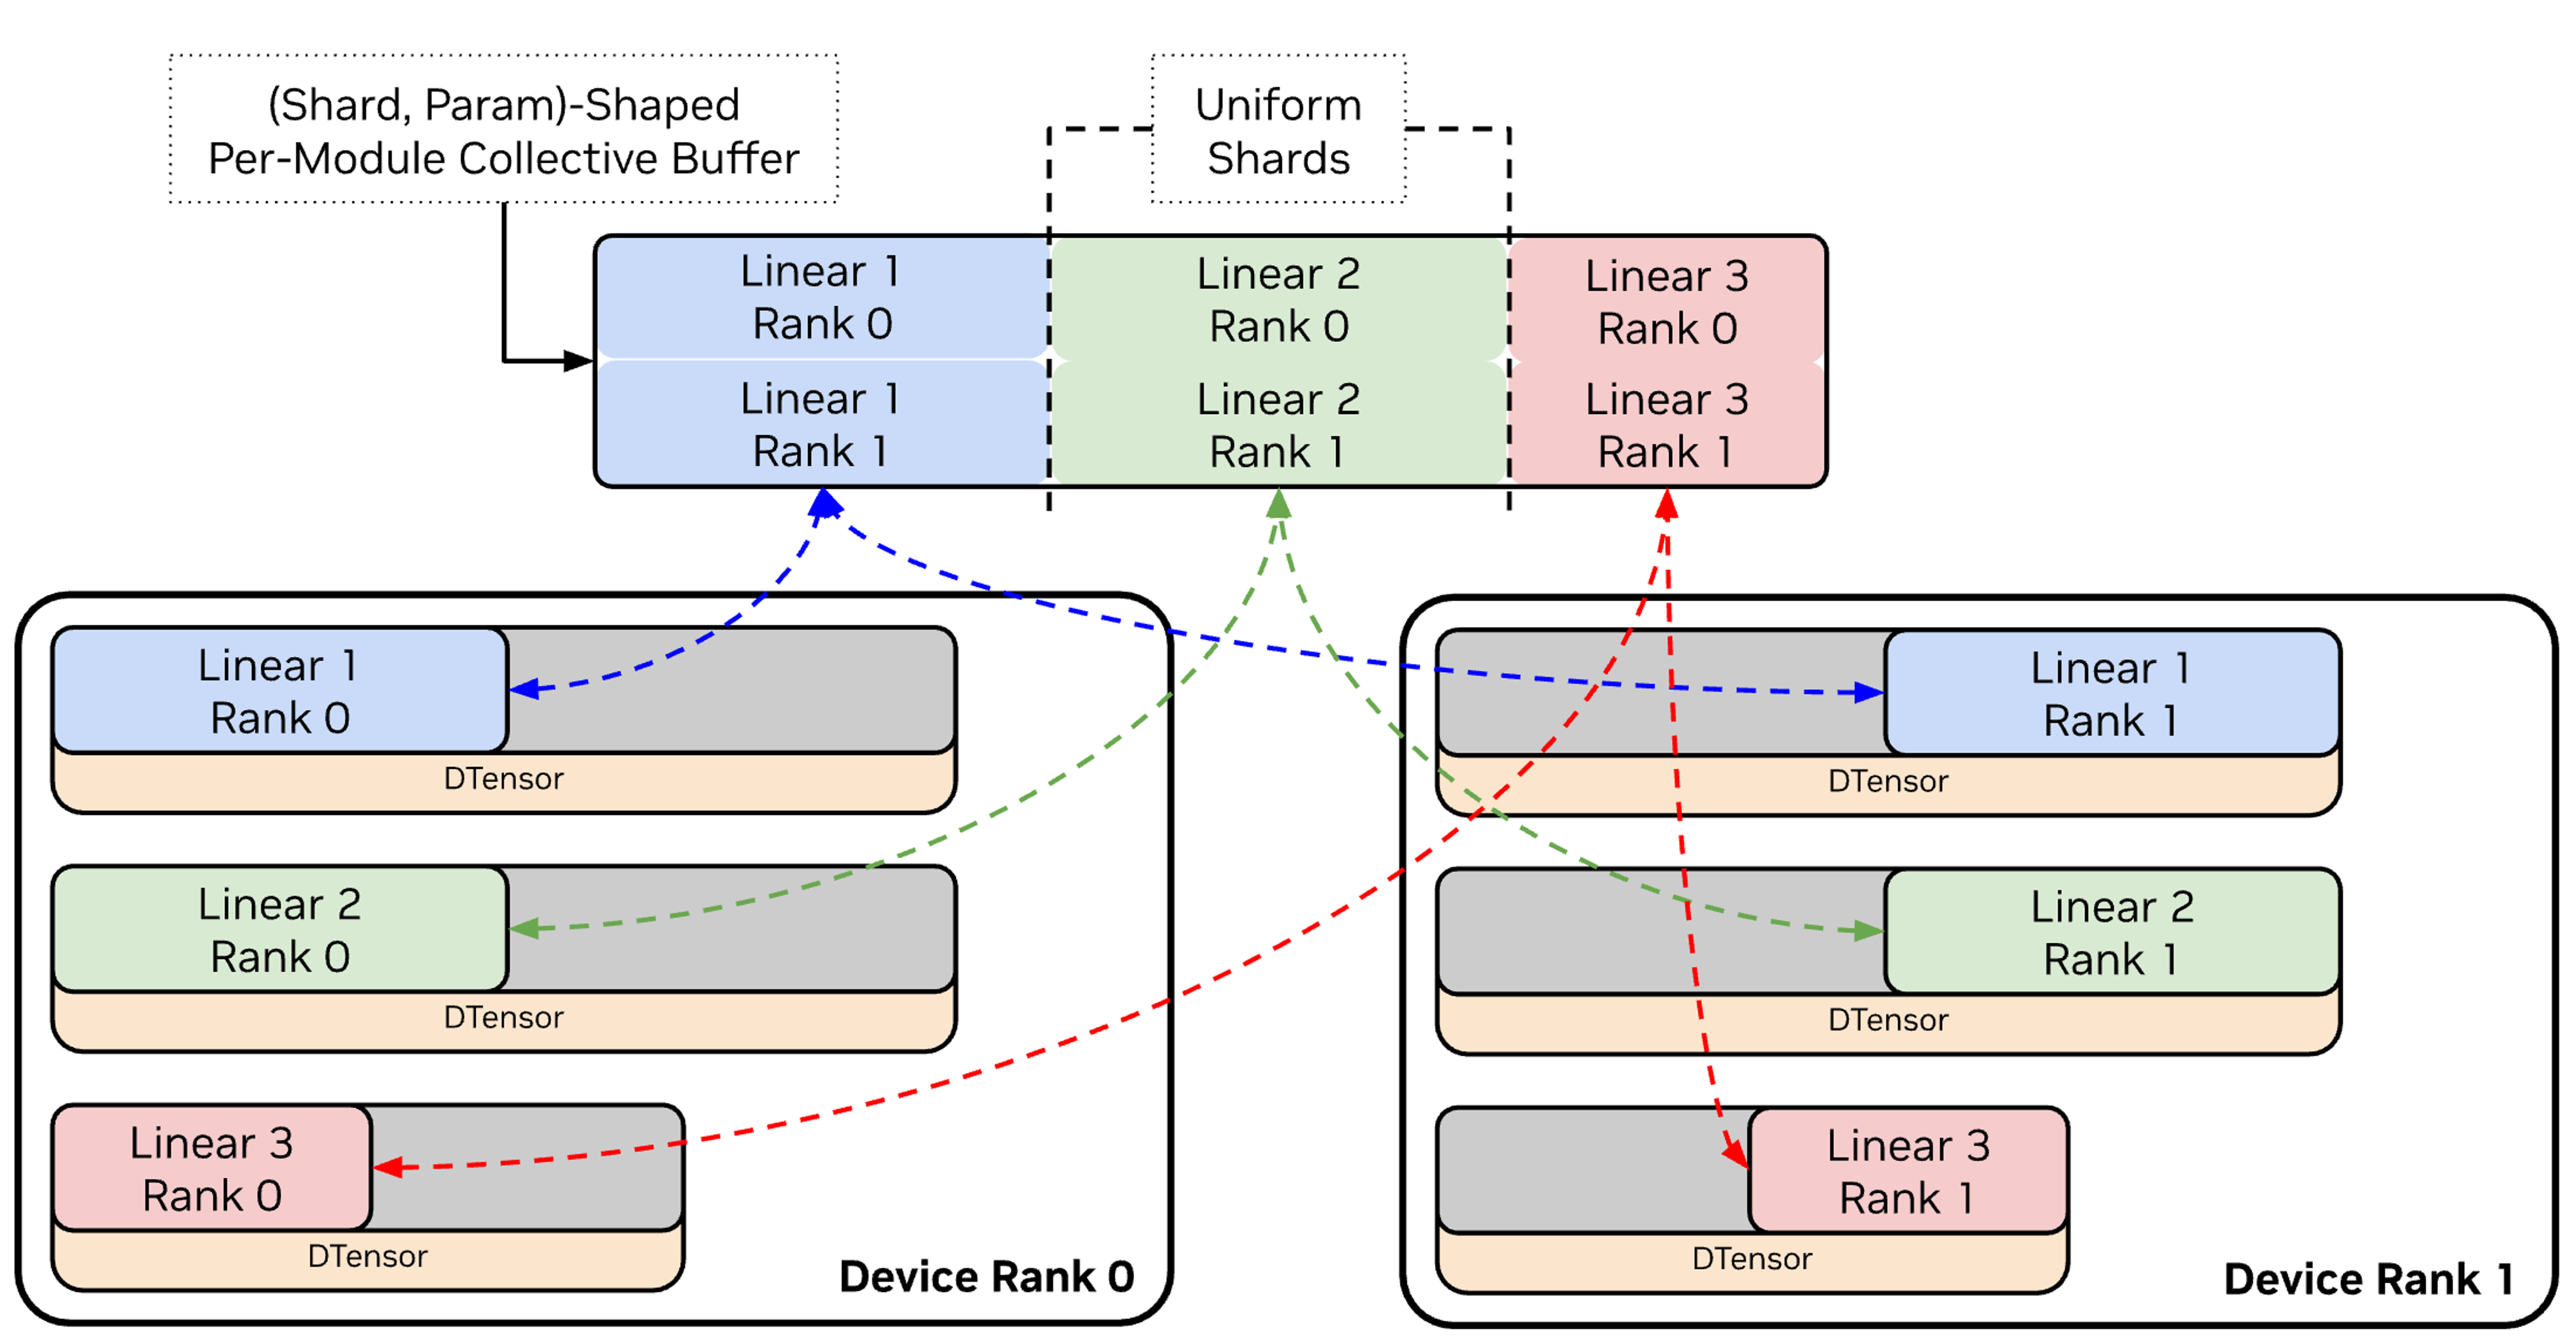
\includegraphics[width=\textwidth]{figures/fsdp2_per_parameter_uniform_sharding.png}
    \caption{FSDP2 按参数均匀分片。}
    \label{fig:fsdp2-sharding}
  \end{subfigure}
  \hfill
  \begin{subfigure}[b]{0.45\textwidth}
    \centering
    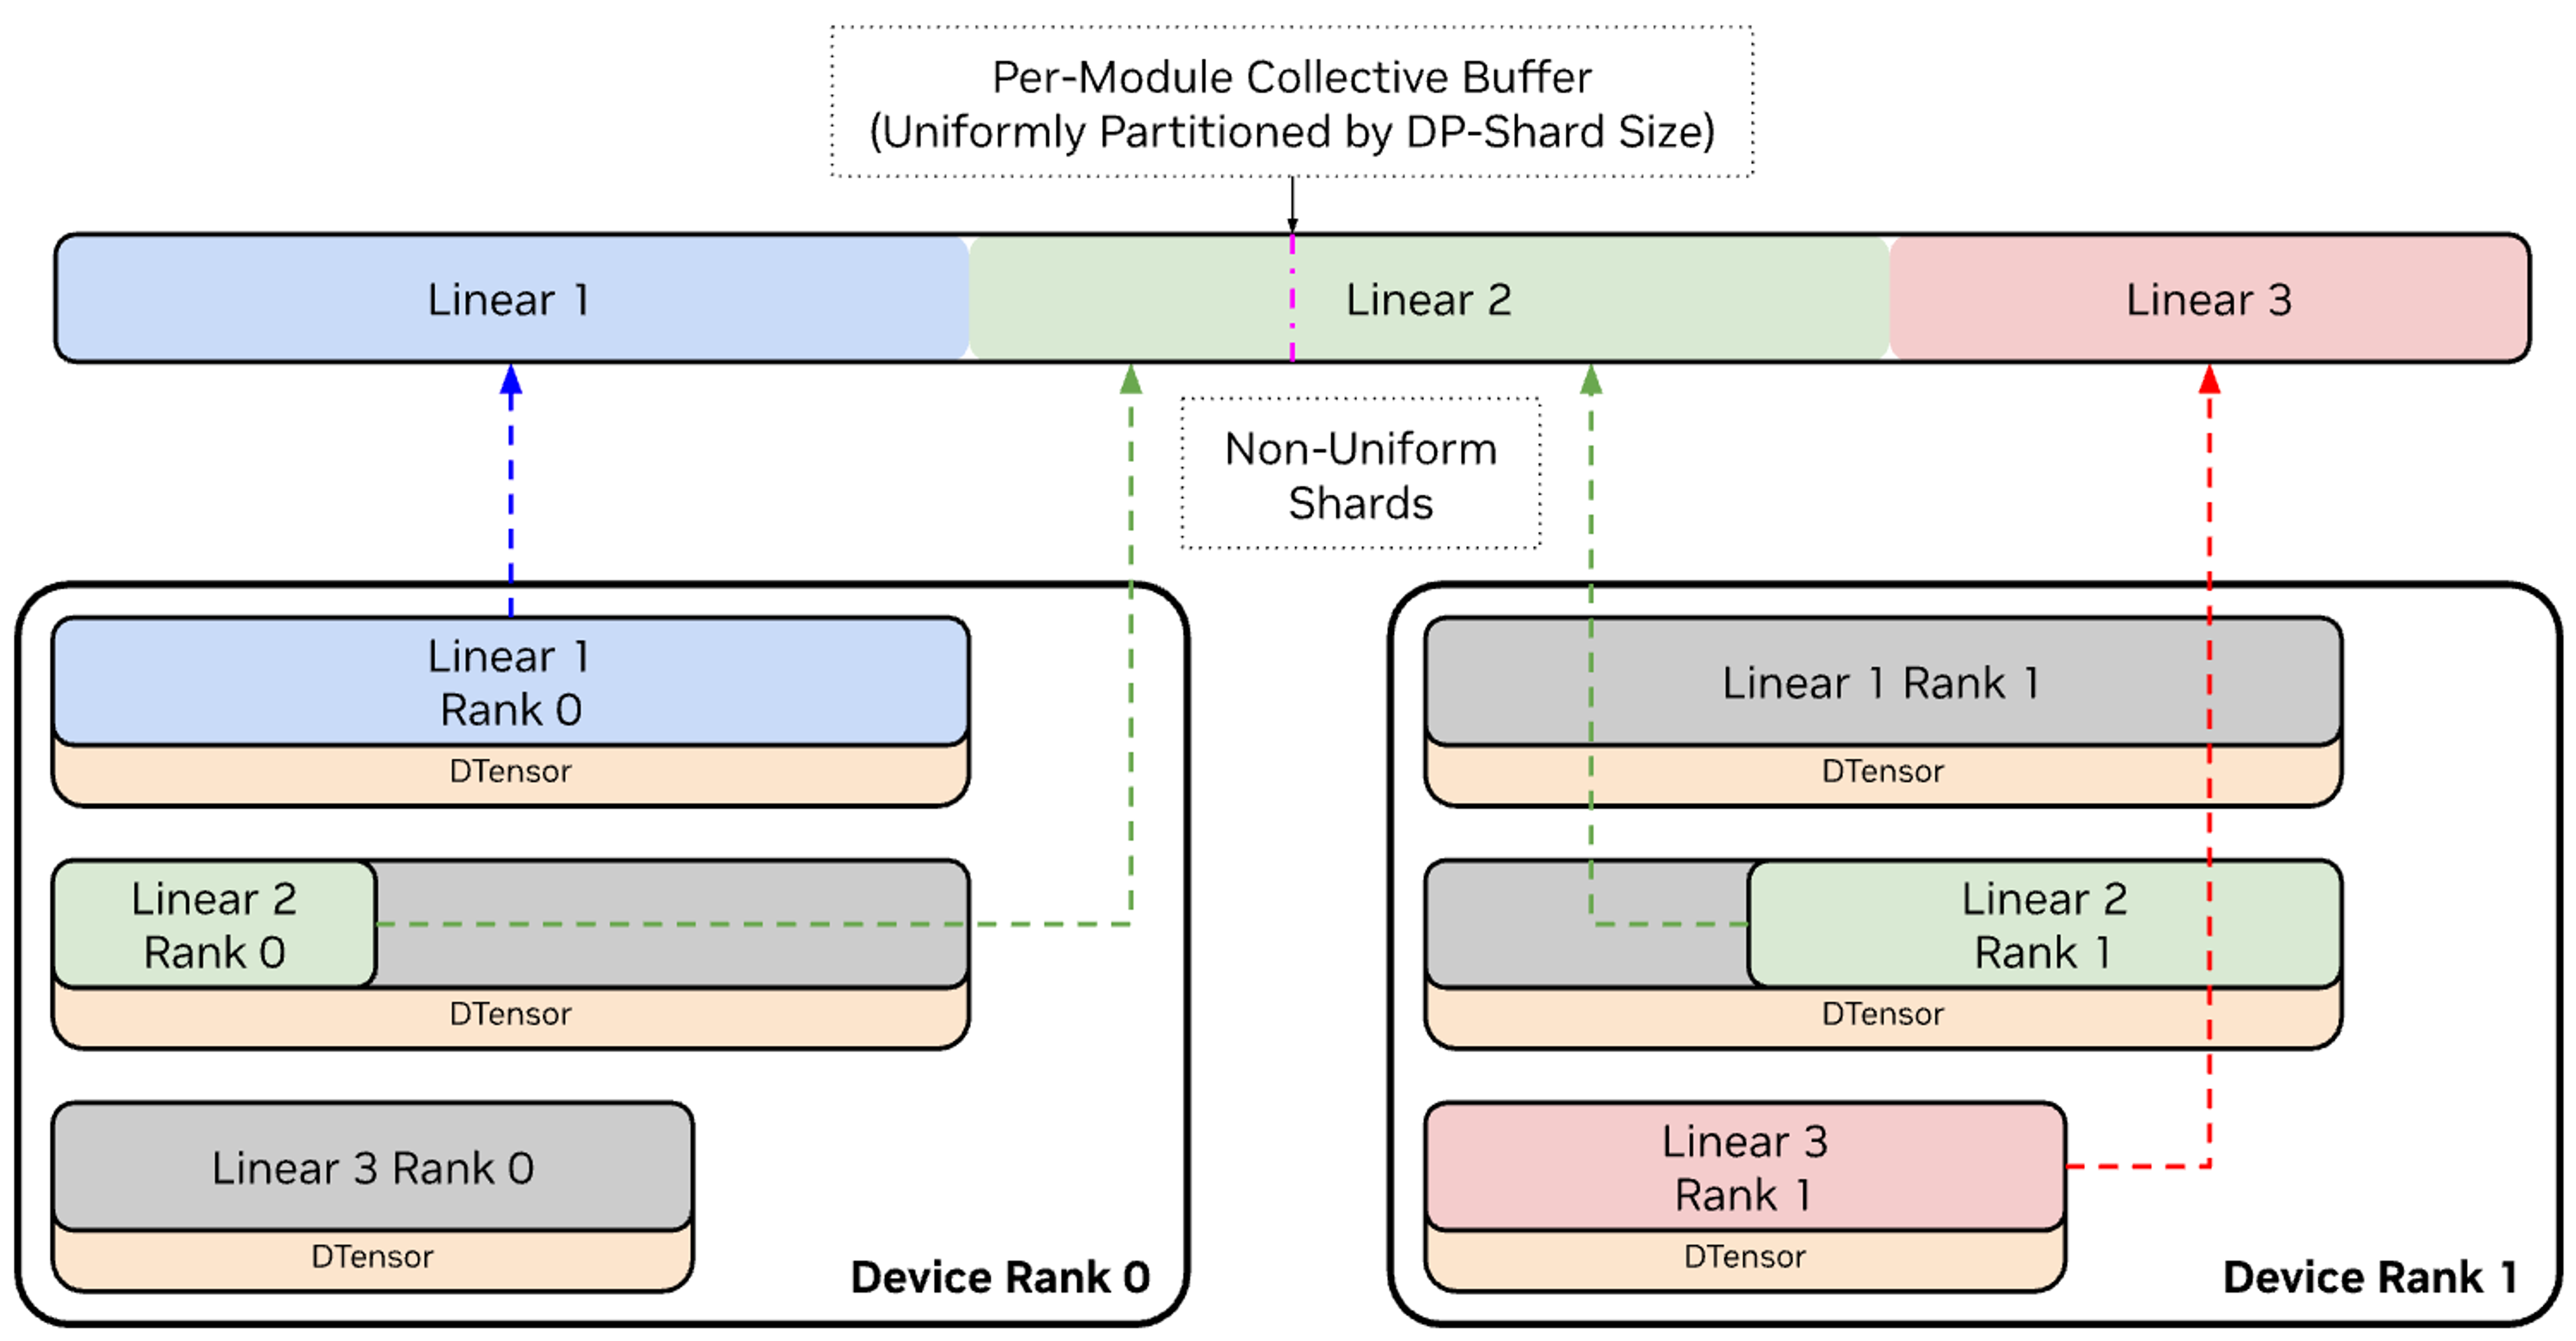
\includegraphics[width=\textwidth]{figures/mfsdp_per_module_non_uniform_sharding.png}
    \caption{Megatron-FSDP 每模块非均匀分片。}
    \label{fig:mfsdp-sharding}
  \end{subfigure}
  \caption{分片策略比较：(a)~FSDP2对各个参数进行统一分片； (b)~Megatron-FSDP 不均匀地展平每个模块和分片，与通信缓冲区对齐。}
  \label{fig:sharding-comparison}
\end{figure}

\textbf{2. 具有 NCCL 用户缓冲区注册的持久双缓冲区：} 基线 FSDP 频繁分配和释放通信缓冲区，NCCL 在每个集合上的用户缓冲区及其内部暂存区域之间复制数据。 Megatron-FSDP 在训练开始时预分配两个持久缓冲区并在它们之间循环（图~\ref{fig:double-buffer}），消除分配流失。 Megatron-FSDP 然后通过用户缓冲区注册 (UBR) 将这些缓冲区注册到 NCCL，因此 NCCL 可以直接读取和写入预先注册的内存，而无需中间副本。综合效果是真正的零拷贝通信。在 NVLink 系统上，通信内核的 SM 占用量从 8--32 个 SM 下降到 1--4 个 SM。在支持 SHARP 的 InfiniBand 上，网络交换机可以完全处理缩减并释放 GPU SM。

\begin{figure}[ht]
  \centering
  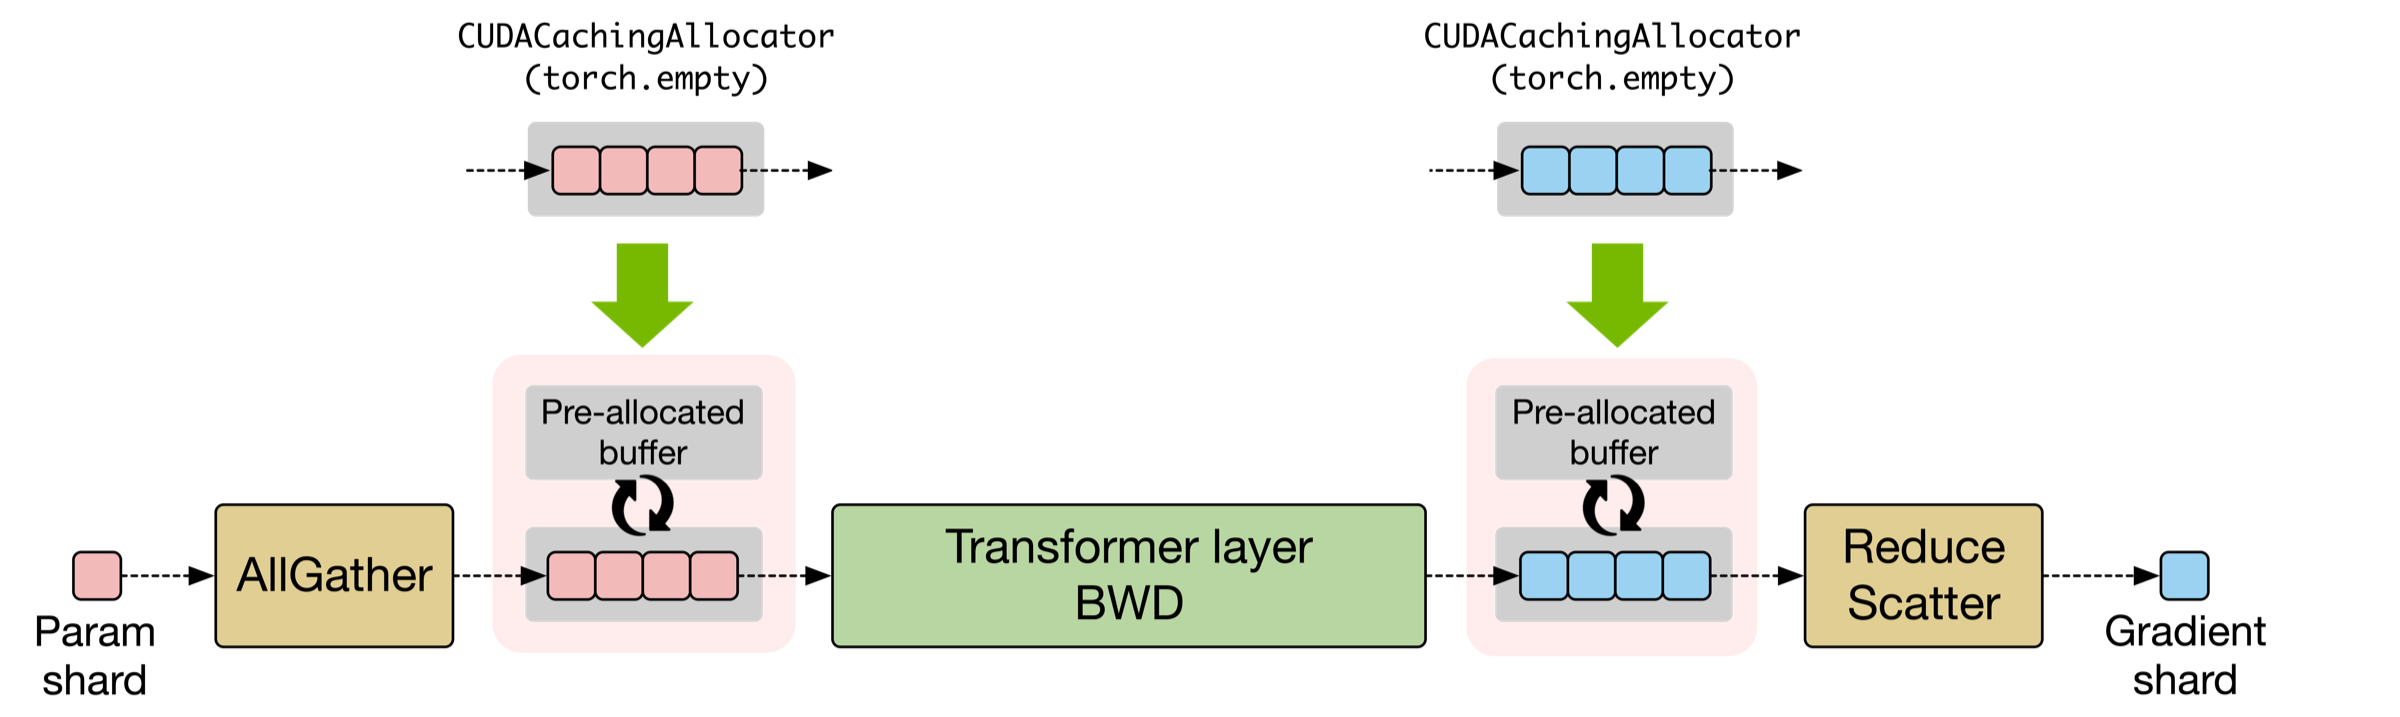
\includegraphics[width=0.85\textwidth]{figures/persistent_double_buffers.png}
  \caption{持久双缓冲区设计：两个预分配缓冲区在 FSDP 集合之间循环，消除了分配开销并启用 NCCL 用户缓冲区注册。}
  \label{fig:double-buffer}
\end{figure}

\paragraph{计算--通信重叠}

即使使用零拷贝集合，AllGather 和ReduceScatter 仍然占用网络，同时GPU 等待参数或梯度同步。 Megatron-FSDP 使用专用 CUDA 流通过计算来管道化这些集合：在当前单元的前向或后向传递仍在执行时发出下一个 FSDP 单元的 AllGather，并且用于梯度的 ReduceScatter 与后续层的后向传递同时运行。增加微批量大小可以扩展可用于隐藏通信的计算窗口，但代价是更高的内存使用量。用户可以通过以下方式调整这种权衡 \texttt{overlap\_param\_gather} 和 \texttt{overlap\_grad\_reduce} 旗帜。

% \paragraph{DTensor-Based Checkpointing}

% Megatron-FSDP represents all model parameters as PyTorch DTensor objects, each carrying a DeviceMesh and Placement that encode its sharding layout. Dense parameters reference the primary DeviceMesh and expert parameters reference the Expert DeviceMesh, so the dual-mesh separation is preserved at the checkpoint level. Checkpointing uses PyTorch's Distributed Checkpoint (DCP) API end-to-end, with no intermediate format conversions. Because DTensor can also express traditional 3D-parallel (TP+PP+DP) layouts, Megatron-FSDP ships conversion tools that translate existing 3D-parallel checkpoints into DTensor-based formats with no manual resharding.

% Summary of memory optimizations
\subsubsection{概括}
表~\ref{tab:memory-opt-summary} 总结了本节中描述的内存优化技术及其主要目标。

\begin{table}[ht]
\centering
\caption{内存优化技术总结。}
\label{tab:memory-opt-summary}
\begin{tabular}{lll}
\toprule
\textbf{技术} & \textbf{内存目标} & \textbf{权衡} \\
\midrule
降低精度训练 & 激活 & 数值精度和 CPU 开销 \\
内存高效排列 & 激活 & - \\
细粒度重新计算 & 激活 & 计算开销 \\
细粒度卸载 & 激活 & CPU 开销和非重叠副本 \\
精度感知优化器 & 优化器状态 & 数值精度 \\
FSDP（含 EP） & 参数+优化器 & 通信开销 \\
\bottomrule
\end{tabular}
\end{table}

这些内存优化相辅相成：内存高效排列以零开销消除冗余存储； FP8/FP4 激活会降低精度，同时对质量影响最小；细粒度重新计算为特定模块提供了有利的计算内存权衡；当其他技术不足时，激活卸载可提供额外的空间；低精度存储和状态卸载减轻了重量并优化了内存； FSDP 可以扩展至超出单设备容量。它们共同将内存从阻塞屏障减少为可管理的约束。

内存优化并不是一个一次性的门，一旦通过就可能被遗忘。对于大规模 MoE 模型，内存在整个优化生命周期中一直是稀缺资源。除了使训练能够继续进行之外，内存空间还可以解锁其他优化：更大的批量大小提供更多的计算来隐藏通信延迟（第~\ref{sec:comm-overlap}），CUDA Graphs需要额外的静态缓冲区（第~\ref{sec:cuda-graphs}），并且 EP 通信重叠必须同时保持多个微批次的激活。以下各节中描述的许多优化都会消耗内存，而上述技术使这种消耗变得可行。

